\documentclass{beamer}
\usepackage[utf8]{inputenc}
\usepackage[UKenglish]{babel}
\usepackage[UKenglish]{isodate}
\usepackage{tikz}
\usepackage{listings}
\usepackage{complexity}
\usepackage{mathtools}
\usepackage{booktabs}

\beamertemplatenavigationsymbolsempty
\usetheme{Rochester}
\usecolortheme{orchid}

\usetikzlibrary{arrows}
\usetikzlibrary{arrows.meta}
\usetikzlibrary{calc}
\usetikzlibrary{positioning}
\usetikzlibrary{shapes}

\newboolean{future}
\setboolean{future}{true}

\author{Paulius Dilkas}
\title{Probabilistic Inference via Weighted Model Counting}
\subtitle{Algorithms, Encodings, and Random Instances}
\date{15th June 2021}

\AtBeginSection[]
{
  \begin{frame}
    \frametitle{Outline}
    \tableofcontents[currentsection]
  \end{frame}
}

\begin{document}

\maketitle

\begin{frame}[fragile]{The Problem of Computing Probability}
  \vspace{-0.75cm}
  \begin{columns}[t]
    \begin{column}{0.65\textwidth}
      \centering
      \begin{block}{ProbLog}
        \vspace{-0.2cm}
        \begin{lstlisting}[basicstyle=\tiny]
0.001 :: burglary.
0.002 :: earthquake.
0.95  :: alarm     :- burglary, earthquake.
0.94  :: alarm     :- burglary, \+ earthquake.
0.29  :: alarm     :- \+ burglary, earthquake.
0.001 :: alarm     :- \+ burglary, \+ earthquake.
0.9   :: johnCalls :- alarm.
0.05  :: johnCalls :- \+ alarm.
0.7   :: maryCalls :- alarm.
0.01  :: maryCalls :- \+ alarm.
        \end{lstlisting}
        \vspace{-0.2cm}
      \end{block}
      \vspace{-0.25cm}
      \begin{block}{BLOG}
        \vspace{-0.2cm}
        \begin{lstlisting}[escapeinside={(*}{*)},basicstyle=\tiny]
random Boolean Burglary (*$\sim$*) BooleanDistrib(0.001);
random Boolean Earthquake (*$\sim$*) BooleanDistrib(0.002);
random Boolean Alarm (*$\sim$*)
  if Burglary then
    if Earthquake then BooleanDistrib(0.95)
    else BooleanDistrib(0.94)
  else
    if Earthquake then BooleanDistrib(0.29)
    else BooleanDistrib(0.001);
random Boolean JohnCalls (*$\sim$*)
  if Alarm then BooleanDistrib(0.9)
  else BooleanDistrib(0.05);
random Boolean MaryCalls (*$\sim$*)
  if Alarm then BooleanDistrib(0.7)
  else BooleanDistrib(0.01);
        \end{lstlisting}
        \vspace{-0.2cm}
      \end{block}
    \end{column}
    \begin{column}{0.35\textwidth}
      \begin{block}{Bayesian Network}
        \centering
        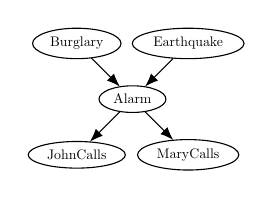
\begin{tikzpicture}[node distance=2cm,scale=0.5,every node/.style={scale=0.5}]
          \node[draw,ellipse] (alarm) {Alarm};
          \node[draw,ellipse,above left of=alarm] (burglary) {Burglary};
          \node[draw,ellipse,above right of=alarm] (earthquake) {Earthquake};
          \node[draw,ellipse,below left of=alarm] (johnCalls) {JohnCalls};
          \node[draw,ellipse,below right of=alarm] (maryCalls) {MaryCalls};
          \draw[-Latex] (burglary) -- (alarm);
          \draw[-Latex] (earthquake) -- (alarm);
          \draw[-Latex] (alarm) -- (johnCalls);
          \draw[-Latex] (alarm) -- (maryCalls);
        \end{tikzpicture}
      \end{block}
      \vspace{1cm}
      \begin{block}{Markov Random Field}
        \centering
        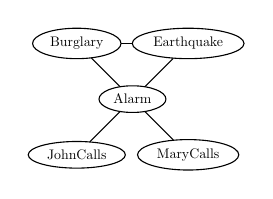
\begin{tikzpicture}[node distance=2cm,scale=0.5,every node/.style={scale=0.5}]
          \node[draw,ellipse] (alarm) {Alarm};
          \node[draw,ellipse,above left of=alarm] (burglary) {Burglary};
          \node[draw,ellipse,above right of=alarm] (earthquake) {Earthquake};
          \node[draw,ellipse,below left of=alarm] (johnCalls) {JohnCalls};
          \node[draw,ellipse,below right of=alarm] (maryCalls) {MaryCalls};
          \draw (burglary) -- (earthquake);
          \draw (burglary) -- (alarm);
          \draw (earthquake) -- (alarm);
          \draw (alarm) -- (johnCalls);
          \draw (alarm) -- (maryCalls);
        \end{tikzpicture}
      \end{block}
    \end{column}
  \end{columns}
  \onslide<2>{
    \begin{tikzpicture}[remember picture,overlay]
      \node[draw,star,fill=red!10] (wmc) at (current page.center) {WMC};
      \coordinate[xshift=-0.25\linewidth,yshift=-0.25\textheight] (p1) at (current page.center);
      \coordinate[xshift=0.25\linewidth,yshift=-0.25\textheight] (p2) at (current page.center);
      \coordinate[xshift=-0.25\linewidth,yshift=0.25\textheight] (p3) at (current page.center);
      \coordinate[xshift=0.25\linewidth,yshift=0.25\textheight] (p4) at (current page.center);
      \draw[-latex,line width=2pt,color=red!50] (p1) -- (wmc);
      \draw[-latex,line width=2pt,color=red!50] (p2) -- (wmc);
      \draw[-latex,line width=2pt,color=red!50] (p3) -- (wmc);
      \draw[-latex,line width=2pt,color=red!50] (p4) -- (wmc);
    \end{tikzpicture}
  }
\end{frame}

\begin{frame}[fragile]{Weighted Model Counting (WMC)}
  \begin{columns}
    \begin{column}{0.5\textwidth}
      \begin{itemize}
      \item Generalises propositional model counting ($\#\SAT{}$)
      \item Applications:
        \begin{itemize}
        \item graphical models
        \item probabilistic programming
        \item neural-symbolic artificial intelligence
        \end{itemize}
      \item Main types of algorithms:
        \begin{itemize}
        \item using knowledge compilation
        \item using a \SAT{} solver
        \item manipulating pseudo-Boolean functions
        \end{itemize}
      \end{itemize}
    \end{column}
    \begin{column}{0.5\textwidth}
      \begin{example}
      $w(x) = 0.3$, $w(\neg x) = 0.7$, $w(y) = 0.2$, $w(\neg y) = 0.8$
      \vspace{1cm}

      $\mathsf{WMC}(\alert{x \lor y}) = w(x)w(y) + w(x)w(\neg y) + w(\neg x)w(y)
      = 0.44$
      \end{example}
    \end{column}
  \end{columns}
\end{frame}

\begin{frame}
  \frametitle{Outline}
  \tableofcontents
\end{frame}

\section{The UAI Paper: Weighted Model Counting with Conditional Weights for Bayesian Networks}

\begin{frame}{An Alternative Way to Think About WMC}
  \begin{itemize}
  \item Let \structure{$V$} be the set of variables.
  \item Then \structure{$2^{2^V}$} is the Boolean algebra of propositional
    formulas.
  \end{itemize}
  \begin{definition}
    A \alert{measure} is a function \structure{$\mu\colon 2^{2^V} \to
      \mathbb{R}_{\ge 0}$} such that:
    \begin{itemize}
    \item \structure{$\mu(\bot) = 0$};
    \item \structure{$\mu(x \lor y) = \mu(x) + \mu(y)$} whenever \structure{$x
        \land y = \bot$}.
    \end{itemize}
  \end{definition}
  \begin{block}{Observation}
    WMC corresponds to the process of calculating the value of
    \structure{$\mu(x)$} for some \structure{$x \in 2^{2^V}$}.
  \end{block}
\end{frame}

\begin{frame}{The Limitations and Capabilities of WMC}
  \begin{alertblock}{Observation}
    Classical WMC is only able to evaluate \structure{factorable} measures
    (c.f., a collection of mutually independent random variables).
  \end{alertblock}
  \begin{theorem}[Informal Version]
    It is always possible to add more variables to turn a non-factorable measure
    into a factorable measure.
  \end{theorem}
  However, that is not necessarily a good idea!
\end{frame}

\begin{frame}{Experimental Results}
  \centering
  \input{../../../published/wmc-without-parameters/doc/long_talk/cumulative2}
\end{frame}

\section{The SAT Paper: Weighted Model Counting Without Parameter Variables}

\begin{frame}{Formalising the Intuition from Before}
  For any propositional formula \structure{$\phi$} over a set of variables
  \structure{$X$} and \structure{$p, q \in \mathbb{R}$}, let
  \structure{$[\phi]^p_q\colon 2^X \to \mathbb{R}$} be the pseudo-Boolean
  function defined as
  \[
    [\phi]^p_q(Y) \coloneqq
    \begin{cases}
      p & \text{if } Y \models \phi \\
      q & \text{otherwise}
    \end{cases}
  \]
  for any \structure{$Y \subseteq X$}.

  \begin{definition}[Pseudo-Boolean Projection (PBP)]
    A \alert{PBP instance} is a tuple \structure{$(F, X, \omega)$}, where
    \structure{$X$} is the set of variables, \structure{$F$} is a set of
    two-valued pseudo-Boolean functions \structure{$2^X \to \mathbb{R}$}, and
    \structure{$\omega \in \mathbb{R}$} is the scaling factor.
  \end{definition}
\end{frame}

\begin{frame}{From WMC to PBP}
  The WMC instance has \structure{$x$} as the only \alert{indicator} variable
  and \structure{$p$}, \structure{$q$} as \alert{parameter} variables with
  weights \structure{$w(p) = 0.2$}, \structure{$w(q) = 0.8$}, and
  \structure{$w(\neg p) = w(\neg q) = 1$}.
  \begin{center}
    \begin{tabular}{llll}
      \toprule
      WMC Clause & \onslide<2->{In CNF} & \onslide<3->{Pseudo-Boolean Function} & \\
      \midrule
      $\neg x \Rightarrow p$ & \onslide<2->{$x \lor p$} & \onslide<3->{$[\neg x]_1^{0.2}$} & \\
      $p \Rightarrow \neg x$ & \onslide<2->{$\neg x \lor \neg p$} & & \onslide<4->{$[x]^{0.8}_{0.2}$} \\
      $x \Rightarrow q$ & \onslide<2->{$\neg x \lor q$} & \onslide<3->{$[x]_1^{0.8}$} & \\
      $q \Rightarrow x$ & \onslide<2->{$x \lor \neg q$} & & \\
      $\neg x$ & \onslide<2->{$\neg x$} & \onslide<3->{$[\neg x]_0^1$} & \onslide<4->{$[\neg x]_0^1$} \\
      \bottomrule
    \end{tabular}
  \end{center}
\end{frame}

\begin{frame}{Experimental Results}
  % Created by tikzDevice version 0.12.3.1 on 2022-06-27 10:59:57
% !TEX encoding = UTF-8 Unicode
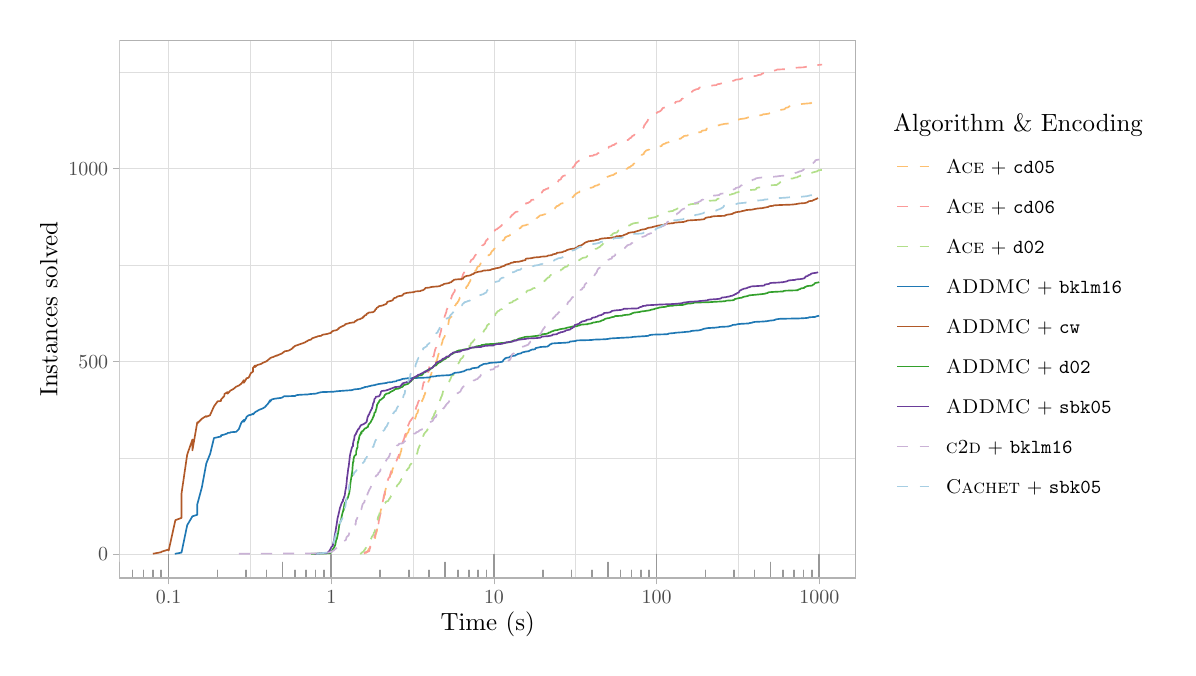
\begin{tikzpicture}[x=1pt,y=1pt]
\definecolor{fillColor}{RGB}{255,255,255}
\path[use as bounding box,fill=fillColor,fill opacity=0.00] (0,0) rectangle (411.94,224.04);
\begin{scope}
\path[clip] (  0.00,  0.00) rectangle (411.94,224.04);
\definecolor{drawColor}{RGB}{255,255,255}
\definecolor{fillColor}{RGB}{255,255,255}

\path[draw=drawColor,line width= 0.5pt,line join=round,line cap=round,fill=fillColor] (  0.00,  0.00) rectangle (411.94,224.04);
\end{scope}
\begin{scope}
\path[clip] ( 33.14, 25.11) rectangle (299.31,219.54);
\definecolor{fillColor}{RGB}{255,255,255}

\path[fill=fillColor] ( 33.14, 25.11) rectangle (299.31,219.54);
\definecolor{drawColor}{gray}{0.87}

\path[draw=drawColor,line width= 0.1pt,line join=round] ( 33.14, 68.65) --
	(299.31, 68.65);

\path[draw=drawColor,line width= 0.1pt,line join=round] ( 33.14,138.35) --
	(299.31,138.35);

\path[draw=drawColor,line width= 0.1pt,line join=round] ( 33.14,208.05) --
	(299.31,208.05);

\path[draw=drawColor,line width= 0.1pt,line join=round] ( 80.33, 25.11) --
	( 80.33,219.54);

\path[draw=drawColor,line width= 0.1pt,line join=round] (139.11, 25.11) --
	(139.11,219.54);

\path[draw=drawColor,line width= 0.1pt,line join=round] (197.89, 25.11) --
	(197.89,219.54);

\path[draw=drawColor,line width= 0.1pt,line join=round] (256.67, 25.11) --
	(256.67,219.54);

\path[draw=drawColor,line width= 0.2pt,line join=round] ( 33.14, 33.80) --
	(299.31, 33.80);

\path[draw=drawColor,line width= 0.2pt,line join=round] ( 33.14,103.50) --
	(299.31,103.50);

\path[draw=drawColor,line width= 0.2pt,line join=round] ( 33.14,173.20) --
	(299.31,173.20);

\path[draw=drawColor,line width= 0.2pt,line join=round] ( 50.94, 25.11) --
	( 50.94,219.54);

\path[draw=drawColor,line width= 0.2pt,line join=round] (109.72, 25.11) --
	(109.72,219.54);

\path[draw=drawColor,line width= 0.2pt,line join=round] (168.50, 25.11) --
	(168.50,219.54);

\path[draw=drawColor,line width= 0.2pt,line join=round] (227.28, 25.11) --
	(227.28,219.54);

\path[draw=drawColor,line width= 0.2pt,line join=round] (286.06, 25.11) --
	(286.06,219.54);
\definecolor{drawColor}{RGB}{253,191,111}

\path[draw=drawColor,line width= 0.6pt,dash pattern=on 4pt off 4pt ,line join=round] (122.04, 34.08) --
	(122.19, 34.22) --
	(122.35, 34.36) --
	(122.66, 34.78) --
	(122.66, 34.50) --
	(122.81, 34.92) --
	(122.96, 35.20) --
	(122.96, 35.06) --
	(123.27, 35.62) --
	(123.27, 35.76) --
	(123.57, 35.90) --
	(123.71, 36.31) --
	(123.86, 36.59) --
	(124.01, 36.73) --
	(124.73, 37.29) --
	(124.73, 37.01) --
	(124.73, 37.43) --
	(124.87, 37.57) --
	(125.01, 37.85) --
	(125.15, 38.13) --
	(125.15, 38.27) --
	(125.43, 38.68) --
	(125.43, 39.38) --
	(125.56, 39.66) --
	(125.56, 39.80) --
	(125.70, 40.50) --
	(125.70, 40.64) --
	(125.84, 41.05) --
	(125.97, 41.47) --
	(126.11, 41.89) --
	(126.24, 42.59) --
	(126.24, 42.45) --
	(126.37, 43.70) --
	(126.51, 44.12) --
	(126.51, 43.98) --
	(126.64, 44.54) --
	(126.77, 44.96) --
	(126.77, 44.82) --
	(126.90, 45.51) --
	(127.03, 46.49) --
	(127.16, 47.47) --
	(127.29, 48.02) --
	(127.42, 48.30) --
	(127.54, 49.42) --
	(127.67, 49.97) --
	(127.80, 50.11) --
	(127.80, 50.53) --
	(127.92, 51.09) --
	(128.05, 51.93) --
	(128.17, 52.34) --
	(128.29, 52.62) --
	(128.29, 52.48) --
	(128.42, 53.18) --
	(128.54, 53.60) --
	(128.66, 53.88) --
	(128.78, 54.57) --
	(128.90, 54.99) --
	(129.02, 55.13) --
	(129.14, 55.41) --
	(129.14, 56.11) --
	(129.26, 56.94) --
	(129.38, 57.36) --
	(129.50, 57.92) --
	(129.62, 58.20) --
	(129.73, 58.62) --
	(129.96, 59.04) --
	(130.08, 59.31) --
	(130.08, 59.45) --
	(130.19, 59.87) --
	(130.31, 60.43) --
	(130.42, 60.85) --
	(130.54, 60.99) --
	(130.65, 61.27) --
	(130.76, 61.41) --
	(130.87, 61.68) --
	(130.98, 62.24) --
	(131.09, 62.52) --
	(131.42, 62.94) --
	(131.53, 63.08) --
	(131.64, 63.22) --
	(131.64, 63.50) --
	(131.75, 63.91) --
	(131.86, 64.61) --
	(131.96, 64.75) --
	(132.07, 64.89) --
	(132.18, 65.17) --
	(132.28, 65.31) --
	(132.49, 65.45) --
	(132.70, 65.59) --
	(132.80, 66.01) --
	(132.91, 66.42) --
	(133.01, 66.70) --
	(133.21, 66.84) --
	(133.32, 66.98) --
	(133.42, 67.12) --
	(133.52, 67.40) --
	(133.72, 67.54) --
	(133.82, 67.68) --
	(134.01, 67.96) --
	(134.11, 68.24) --
	(134.21, 68.38) --
	(134.31, 68.93) --
	(134.41, 69.35) --
	(134.50, 69.63) --
	(134.60, 69.77) --
	(134.60, 70.05) --
	(134.70, 70.19) --
	(134.79, 70.61) --
	(134.98, 71.16) --
	(135.08, 71.86) --
	(135.17, 72.56) --
	(135.27, 72.70) --
	(135.36, 73.11) --
	(135.45, 73.67) --
	(135.55, 73.81) --
	(135.64, 74.09) --
	(135.73, 74.23) --
	(135.91, 74.65) --
	(136.01, 74.93) --
	(136.10, 75.21) --
	(136.28, 75.48) --
	(136.37, 75.62) --
	(136.46, 75.76) --
	(136.55, 76.18) --
	(136.64, 76.32) --
	(136.72, 76.60) --
	(136.90, 76.88) --
	(136.99, 77.16) --
	(137.08, 77.44) --
	(137.25, 77.58) --
	(137.42, 77.71) --
	(137.51, 77.85) --
	(137.68, 78.41) --
	(137.77, 78.83) --
	(138.02, 78.97) --
	(138.10, 79.25) --
	(138.19, 79.67) --
	(138.36, 79.81) --
	(138.36, 79.95) --
	(138.52, 80.08) --
	(138.60, 80.22) --
	(138.77, 80.36) --
	(138.85, 80.50) --
	(138.93, 80.64) --
	(139.01, 80.78) --
	(139.09, 80.92) --
	(139.17, 81.20) --
	(139.25, 81.48) --
	(139.25, 81.34) --
	(139.33, 81.62) --
	(139.41, 81.76) --
	(139.57, 81.90) --
	(139.65, 82.04) --
	(139.65, 82.18) --
	(139.73, 82.31) --
	(139.81, 82.45) --
	(139.89, 82.59) --
	(139.97, 82.73) --
	(140.04, 82.87) --
	(140.20, 83.43) --
	(140.28, 83.57) --
	(140.35, 83.71) --
	(140.43, 84.27) --
	(140.51, 84.41) --
	(140.58, 84.55) --
	(140.74, 84.68) --
	(140.89, 84.82) --
	(140.89, 84.96) --
	(140.96, 85.10) --
	(140.96, 85.38) --
	(141.04, 85.52) --
	(141.11, 85.66) --
	(141.19, 85.94) --
	(141.19, 86.08) --
	(141.41, 86.22) --
	(141.48, 86.36) --
	(141.56, 86.50) --
	(141.70, 87.05) --
	(141.77, 87.19) --
	(141.77, 87.33) --
	(141.92, 87.47) --
	(141.99, 87.61) --
	(142.14, 87.89) --
	(142.14, 88.03) --
	(142.28, 88.17) --
	(142.35, 88.45) --
	(142.42, 88.87) --
	(142.42, 88.59) --
	(142.49, 89.28) --
	(142.49, 89.01) --
	(142.63, 89.42) --
	(142.77, 89.70) --
	(142.91, 90.12) --
	(143.05, 90.26) --
	(143.12, 90.40) --
	(143.12, 90.96) --
	(143.33, 91.10) --
	(143.46, 91.38) --
	(143.53, 91.65) --
	(143.60, 91.93) --
	(143.60, 92.07) --
	(143.80, 92.21) --
	(143.94, 92.35) --
	(143.94, 92.49) --
	(144.07, 92.91) --
	(144.13, 93.19) --
	(144.20, 93.47) --
	(144.27, 94.16) --
	(144.33, 94.44) --
	(144.40, 94.72) --
	(144.40, 94.86) --
	(144.46, 95.00) --
	(144.53, 95.14) --
	(144.59, 95.28) --
	(144.66, 95.70) --
	(144.66, 95.56) --
	(144.72, 95.84) --
	(144.79, 96.12) --
	(144.85, 96.25) --
	(144.92, 96.39) --
	(144.98, 96.53) --
	(145.11, 96.67) --
	(145.17, 96.95) --
	(145.24, 97.09) --
	(145.30, 97.23) --
	(145.30, 97.51) --
	(145.36, 97.79) --
	(145.49, 98.07) --
	(145.55, 98.21) --
	(145.62, 98.35) --
	(145.68, 98.62) --
	(145.80, 98.76) --
	(145.87, 99.04) --
	(145.93, 99.32) --
	(146.05, 99.60) --
	(146.17, 99.88) --
	(146.23,100.02) --
	(146.36,100.30) --
	(146.42,100.44) --
	(146.48,100.58) --
	(146.54,100.99) --
	(146.66,101.13) --
	(146.72,101.55) --
	(146.78,101.69) --
	(146.84,101.83) --
	(146.96,101.97) --
	(147.02,102.25) --
	(147.02,102.11) --
	(147.08,102.39) --
	(147.19,102.81) --
	(147.43,103.08) --
	(147.49,103.22) --
	(147.54,103.36) --
	(147.66,103.50) --
	(147.83,103.78) --
	(147.95,104.06) --
	(147.95,104.20) --
	(148.06,104.62) --
	(148.17,105.04) --
	(148.23,105.18) --
	(148.29,105.45) --
	(148.29,105.32) --
	(148.34,105.87) --
	(148.46,106.01) --
	(148.51,106.15) --
	(148.57,106.29) --
	(148.62,106.43) --
	(148.68,106.71) --
	(148.73,106.85) --
	(148.79,106.99) --
	(148.90,107.27) --
	(148.90,107.13) --
	(149.01,107.41) --
	(149.06,107.82) --
	(149.12,107.96) --
	(149.23,108.10) --
	(149.28,108.24) --
	(149.34,108.80) --
	(149.34,108.38) --
	(149.44,108.94) --
	(149.50,109.36) --
	(149.55,109.50) --
	(149.60,109.78) --
	(149.66,109.92) --
	(149.71,110.05) --
	(149.76,110.19) --
	(149.82,110.33) --
	(149.87,110.61) --
	(149.98,111.17) --
	(150.03,111.31) --
	(150.13,111.45) --
	(150.19,111.59) --
	(150.24,111.73) --
	(150.34,111.87) --
	(150.45,112.01) --
	(150.50,112.15) --
	(150.60,112.29) --
	(150.65,112.42) --
	(150.76,112.70) --
	(150.81,112.98) --
	(150.86,113.12) --
	(150.91,113.40) --
	(151.01,113.54) --
	(151.06,113.68) --
	(151.11,113.82) --
	(151.16,113.96) --
	(151.21,114.24) --
	(151.26,114.38) --
	(151.36,114.65) --
	(151.41,115.07) --
	(151.51,115.21) --
	(151.56,115.35) --
	(151.61,115.49) --
	(151.66,115.77) --
	(151.76,116.05) --
	(151.81,116.19) --
	(151.86,116.33) --
	(151.91,116.61) --
	(151.96,116.75) --
	(152.05,117.16) --
	(152.10,117.44) --
	(152.15,117.86) --
	(152.15,117.58) --
	(152.20,118.28) --
	(152.25,118.42) --
	(152.29,118.56) --
	(152.34,118.70) --
	(152.44,118.84) --
	(152.49,118.98) --
	(152.58,119.12) --
	(152.87,119.39) --
	(152.96,119.53) --
	(153.24,119.67) --
	(153.29,119.81) --
	(153.33,119.95) --
	(153.38,120.23) --
	(153.43,120.37) --
	(153.52,120.51) --
	(153.56,120.65) --
	(153.61,120.79) --
	(153.65,120.93) --
	(153.70,121.21) --
	(153.75,121.35) --
	(153.79,121.49) --
	(153.88,121.62) --
	(153.93,121.76) --
	(153.97,121.90) --
	(154.06,122.32) --
	(154.11,122.74) --
	(154.15,123.02) --
	(154.24,123.30) --
	(154.29,123.44) --
	(154.37,123.58) --
	(154.60,123.72) --
	(154.68,123.86) --
	(154.77,124.13) --
	(154.90,124.27) --
	(155.20,124.55) --
	(155.20,124.41) --
	(155.29,124.69) --
	(155.38,124.83) --
	(155.42,124.97) --
	(155.59,125.11) --
	(155.67,125.25) --
	(155.76,125.39) --
	(155.80,125.53) --
	(155.84,125.67) --
	(155.97,125.95) --
	(156.05,126.09) --
	(156.09,126.22) --
	(156.09,126.36) --
	(156.13,126.50) --
	(156.26,126.64) --
	(156.30,126.78) --
	(156.46,126.92) --
	(156.59,127.06) --
	(156.83,127.20) --
	(156.91,127.34) --
	(156.99,127.62) --
	(157.11,127.76) --
	(157.19,127.90) --
	(157.31,128.18) --
	(157.35,128.32) --
	(157.43,128.46) --
	(157.54,128.59) --
	(157.58,128.73) --
	(157.62,129.01) --
	(157.74,129.15) --
	(158.13,129.29) --
	(158.20,129.43) --
	(158.24,129.57) --
	(158.35,129.71) --
	(158.39,129.85) --
	(158.39,129.99) --
	(158.47,130.13) --
	(158.54,130.27) --
	(158.54,130.41) --
	(158.73,130.55) --
	(158.88,130.69) --
	(158.92,130.82) --
	(159.14,130.96) --
	(159.18,131.10) --
	(159.25,131.38) --
	(159.36,131.52) --
	(159.40,131.66) --
	(159.47,131.80) --
	(159.54,131.94) --
	(159.69,132.08) --
	(159.76,132.22) --
	(159.79,132.36) --
	(159.94,132.50) --
	(159.97,132.64) --
	(160.01,132.92) --
	(160.04,133.06) --
	(160.12,133.19) --
	(160.15,133.33) --
	(160.19,133.47) --
	(160.22,133.61) --
	(160.26,133.75) --
	(160.29,133.89) --
	(160.40,134.03) --
	(160.47,134.17) --
	(160.85,134.31) --
	(160.92,134.59) --
	(161.19,134.87) --
	(161.23,135.01) --
	(161.29,135.15) --
	(161.50,135.29) --
	(161.56,135.56) --
	(161.56,135.43) --
	(161.63,135.84) --
	(161.63,135.70) --
	(161.66,135.98) --
	(161.70,136.12) --
	(161.76,136.26) --
	(162.06,136.40) --
	(162.13,136.54) --
	(162.13,136.68) --
	(162.26,136.82) --
	(162.29,136.96) --
	(162.29,137.10) --
	(162.39,137.24) --
	(162.42,137.38) --
	(162.52,137.52) --
	(162.68,137.66) --
	(163.09,137.79) --
	(163.22,137.93) --
	(163.31,138.07) --
	(163.37,138.21) --
	(163.44,138.35) --
	(163.56,138.49) --
	(163.59,138.63) --
	(163.65,138.77) --
	(163.68,138.91) --
	(163.75,139.05) --
	(163.78,139.19) --
	(163.84,139.33) --
	(164.05,139.47) --
	(164.14,139.61) --
	(164.29,139.75) --
	(164.44,139.89) --
	(164.68,140.03) --
	(164.71,140.16) --
	(164.74,140.44) --
	(164.80,140.58) --
	(165.35,140.72) --
	(165.50,140.86) --
	(165.61,141.00) --
	(165.64,141.28) --
	(165.95,141.42) --
	(166.07,141.56) --
	(166.09,141.70) --
	(166.70,141.84) --
	(166.81,141.98) --
	(167.06,142.12) --
	(167.33,142.26) --
	(167.35,142.39) --
	(167.38,142.53) --
	(167.41,142.67) --
	(167.51,142.81) --
	(167.59,142.95) --
	(167.67,143.09) --
	(167.70,143.23) --
	(167.93,143.37) --
	(168.12,143.51) --
	(168.22,143.65) --
	(168.35,143.79) --
	(168.40,143.93) --
	(168.55,144.07) --
	(168.71,144.21) --
	(168.76,144.35) --
	(168.78,144.63) --
	(168.83,144.76) --
	(168.91,144.90) --
	(169.01,145.04) --
	(169.13,145.18) --
	(169.18,145.32) --
	(169.23,145.46) --
	(169.40,145.60) --
	(169.53,145.74) --
	(169.75,145.88) --
	(170.01,146.02) --
	(170.70,146.16) --
	(170.89,146.30) --
	(170.96,146.44) --
	(171.35,146.58) --
	(171.39,146.72) --
	(171.53,146.86) --
	(171.60,146.99) --
	(171.67,147.13) --
	(172.03,147.27) --
	(172.22,147.55) --
	(172.29,147.69) --
	(172.38,147.83) --
	(172.42,147.97) --
	(172.44,148.11) --
	(172.55,148.25) --
	(172.86,148.39) --
	(173.05,148.53) --
	(173.37,148.67) --
	(173.89,148.81) --
	(174.10,148.95) --
	(174.30,149.09) --
	(174.40,149.23) --
	(174.76,149.36) --
	(174.80,149.50) --
	(175.06,149.64) --
	(175.08,149.78) --
	(175.14,149.92) --
	(175.20,150.06) --
	(175.43,150.34) --
	(176.05,150.48) --
	(176.30,150.62) --
	(176.59,150.76) --
	(176.74,150.90) --
	(176.76,151.04) --
	(177.20,151.18) --
	(177.33,151.32) --
	(177.47,151.46) --
	(177.95,151.60) --
	(178.22,151.73) --
	(178.25,151.87) --
	(178.34,152.01) --
	(178.58,152.15) --
	(178.63,152.29) --
	(178.75,152.43) --
	(179.52,152.57) --
	(180.11,152.71) --
	(180.26,152.85) --
	(182.11,152.99) --
	(182.18,153.13) --
	(182.35,153.27) --
	(182.36,153.41) --
	(182.48,153.55) --
	(182.61,153.69) --
	(182.71,153.96) --
	(183.01,154.10) --
	(183.18,154.24) --
	(183.38,154.38) --
	(183.39,154.52) --
	(183.62,154.66) --
	(183.82,154.80) --
	(183.85,154.94) --
	(183.86,155.08) --
	(183.97,155.22) --
	(184.19,155.36) --
	(184.23,155.50) --
	(184.63,155.64) --
	(184.67,155.78) --
	(184.87,155.92) --
	(184.97,156.06) --
	(185.17,156.20) --
	(185.99,156.33) --
	(186.35,156.47) --
	(186.88,156.61) --
	(187.09,156.75) --
	(187.10,156.89) --
	(187.14,157.03) --
	(187.17,157.17) --
	(187.33,157.31) --
	(187.77,157.45) --
	(187.80,157.59) --
	(188.37,157.73) --
	(189.18,157.87) --
	(189.32,158.01) --
	(189.45,158.15) --
	(189.79,158.29) --
	(189.88,158.43) --
	(190.34,158.56) --
	(190.50,158.70) --
	(190.57,158.84) --
	(190.62,158.98) --
	(190.82,159.12) --
	(190.96,159.26) --
	(191.01,159.40) --
	(191.13,159.54) --
	(191.74,159.68) --
	(191.91,159.82) --
	(192.04,159.96) --
	(192.15,160.10) --
	(192.44,160.24) --
	(192.60,160.38) --
	(192.85,160.52) --
	(193.66,160.66) --
	(193.74,160.80) --
	(194.11,160.93) --
	(194.24,161.07) --
	(194.34,161.21) --
	(194.47,161.35) --
	(194.53,161.49) --
	(194.63,161.63) --
	(194.64,161.77) --
	(194.72,161.91) --
	(195.35,162.05) --
	(195.66,162.19) --
	(195.69,162.33) --
	(195.80,162.47) --
	(196.34,162.61) --
	(196.84,162.75) --
	(197.18,162.89) --
	(197.19,163.03) --
	(197.34,163.16) --
	(197.40,163.30) --
	(197.50,163.44) --
	(197.66,163.58) --
	(197.86,163.72) --
	(197.88,163.86) --
	(198.04,164.00) --
	(198.41,164.14) --
	(198.60,164.28) --
	(198.69,164.42) --
	(199.34,164.56) --
	(199.35,164.70) --
	(199.43,164.84) --
	(200.78,164.98) --
	(200.98,165.12) --
	(201.04,165.26) --
	(201.58,165.40) --
	(201.69,165.53) --
	(201.75,165.67) --
	(202.73,165.95) --
	(202.74,166.09) --
	(203.80,166.23) --
	(204.14,166.37) --
	(204.57,166.51) --
	(204.64,166.65) --
	(204.83,166.79) --
	(205.25,166.93) --
	(205.87,167.07) --
	(206.08,167.21) --
	(206.22,167.35) --
	(207.09,167.49) --
	(207.16,167.63) --
	(207.21,167.77) --
	(207.77,167.90) --
	(207.85,168.04) --
	(207.95,168.18) --
	(208.04,168.32) --
	(208.36,168.46) --
	(208.36,168.60) --
	(208.38,168.74) --
	(208.60,168.88) --
	(208.84,169.02) --
	(208.91,169.16) --
	(208.92,169.30) --
	(208.93,169.44) --
	(209.04,169.58) --
	(209.24,169.72) --
	(209.27,169.86) --
	(209.39,170.00) --
	(209.58,170.13) --
	(209.80,170.27) --
	(210.19,170.41) --
	(210.64,170.55) --
	(210.95,170.69) --
	(211.70,170.83) --
	(211.82,170.97) --
	(212.05,171.11) --
	(212.15,171.25) --
	(212.63,171.39) --
	(212.65,171.53) --
	(213.87,171.67) --
	(213.90,171.81) --
	(214.48,171.95) --
	(214.93,172.09) --
	(214.95,172.23) --
	(215.13,172.37) --
	(216.12,172.50) --
	(216.13,172.64) --
	(216.36,172.78) --
	(216.41,172.92) --
	(216.54,173.06) --
	(216.71,173.20) --
	(216.91,173.34) --
	(217.14,173.48) --
	(217.23,173.62) --
	(217.84,173.76) --
	(217.90,173.90) --
	(218.05,174.04) --
	(218.19,174.18) --
	(218.64,174.32) --
	(218.72,174.46) --
	(218.79,174.60) --
	(218.82,174.73) --
	(219.04,174.87) --
	(219.22,175.01) --
	(219.37,175.15) --
	(219.43,175.29) --
	(220.00,175.43) --
	(220.16,175.57) --
	(220.19,175.71) --
	(220.30,175.85) --
	(220.69,175.99) --
	(220.75,176.13) --
	(220.78,176.27) --
	(220.78,176.41) --
	(220.86,176.55) --
	(221.04,176.69) --
	(221.05,176.83) --
	(221.12,176.97) --
	(221.12,177.10) --
	(221.32,177.24) --
	(221.35,177.38) --
	(221.49,177.52) --
	(221.59,177.66) --
	(221.75,177.80) --
	(221.80,177.94) --
	(221.96,178.08) --
	(222.16,178.22) --
	(222.62,178.36) --
	(222.63,178.50) --
	(222.67,178.64) --
	(222.72,178.78) --
	(222.85,178.92) --
	(222.88,179.06) --
	(223.04,179.20) --
	(223.20,179.33) --
	(223.30,179.47) --
	(223.45,179.61) --
	(223.70,179.75) --
	(224.30,179.89) --
	(224.61,180.03) --
	(224.70,180.17) --
	(224.73,180.31) --
	(225.38,180.45) --
	(226.56,180.59) --
	(227.67,180.73) --
	(228.16,180.87) --
	(228.22,181.01) --
	(228.34,181.15) --
	(229.15,181.29) --
	(229.16,181.43) --
	(229.22,181.57) --
	(229.30,181.70) --
	(229.54,181.84) --
	(229.80,181.98) --
	(230.27,182.12) --
	(230.54,182.26) --
	(230.63,182.40) --
	(231.26,182.54) --
	(231.64,182.68) --
	(231.83,182.82) --
	(231.98,182.96) --
	(233.15,183.10) --
	(233.18,183.24) --
	(233.75,183.38) --
	(234.03,183.52) --
	(234.03,183.66) --
	(234.06,183.80) --
	(236.10,183.94) --
	(236.14,184.07) --
	(236.25,184.21) --
	(236.45,184.35) --
	(236.60,184.49) --
	(236.96,184.63) --
	(237.03,184.77) --
	(237.17,184.91) --
	(238.46,185.05) --
	(238.50,185.19) --
	(239.22,185.33) --
	(239.23,185.47) --
	(239.92,185.61) --
	(239.93,185.75) --
	(240.07,185.89) --
	(240.88,186.03) --
	(241.33,186.17) --
	(243.29,186.30) --
	(243.43,186.44) --
	(243.44,186.58) --
	(243.62,186.72) --
	(243.96,186.86) --
	(245.09,187.00) --
	(245.22,187.14) --
	(245.23,187.28) --
	(245.28,187.42) --
	(245.30,187.56) --
	(246.32,187.70) --
	(246.93,187.84) --
	(247.95,187.98) --
	(248.26,188.12) --
	(248.28,188.26) --
	(248.62,188.40) --
	(248.83,188.54) --
	(249.17,188.67) --
	(250.02,188.81) --
	(250.15,188.95) --
	(251.11,189.09) --
	(251.48,189.23) --
	(252.93,189.37) --
	(253.60,189.51) --
	(253.60,189.65) --
	(254.80,189.79) --
	(255.76,189.93) --
	(255.92,190.07) --
	(255.93,190.21) --
	(256.12,190.35) --
	(256.25,190.49) --
	(256.41,190.63) --
	(256.85,190.77) --
	(256.98,190.90) --
	(257.63,191.04) --
	(258.81,191.18) --
	(259.49,191.32) --
	(259.92,191.46) --
	(260.28,191.60) --
	(260.90,191.74) --
	(261.05,191.88) --
	(261.95,192.02) --
	(263.74,192.16) --
	(263.78,192.30) --
	(265.34,192.44) --
	(265.42,192.58) --
	(265.77,192.72) --
	(267.13,192.86) --
	(267.87,193.00) --
	(268.09,193.14) --
	(268.96,193.27) --
	(269.77,193.41) --
	(269.92,193.55) --
	(270.21,193.69) --
	(270.51,193.83) --
	(270.69,193.97) --
	(271.01,194.11) --
	(271.86,194.25) --
	(272.47,194.39) --
	(273.35,194.53) --
	(273.61,194.67) --
	(273.72,194.81) --
	(273.87,194.95) --
	(273.93,195.09) --
	(274.75,195.23) --
	(274.96,195.37) --
	(275.05,195.51) --
	(275.22,195.64) --
	(276.02,195.78) --
	(276.55,195.92) --
	(276.71,196.06) --
	(278.34,196.20) --
	(279.04,196.34) --
	(279.88,196.48) --
	(281.39,196.62) --
	(283.09,196.76) --
	(283.15,196.90) --
	(283.32,197.04) --
	(284.14,197.18) --
	(284.32,197.32) --
	(284.84,197.46) --
	(285.42,197.60) --
	(285.90,197.74);
\definecolor{drawColor}{RGB}{251,154,153}

\path[draw=drawColor,line width= 0.6pt,dash pattern=on 4pt off 4pt ,line join=round] (121.56, 33.94) --
	(121.72, 34.08) --
	(121.88, 34.36) --
	(122.04, 34.50) --
	(122.66, 34.64) --
	(123.27, 34.78) --
	(123.42, 34.92) --
	(123.57, 35.62) --
	(123.71, 36.04) --
	(123.86, 36.59) --
	(124.01, 36.73) --
	(124.15, 37.01) --
	(124.15, 36.87) --
	(124.30, 37.29) --
	(124.44, 37.57) --
	(124.44, 37.43) --
	(124.58, 38.13) --
	(124.73, 38.40) --
	(124.87, 38.68) --
	(125.01, 39.38) --
	(125.15, 39.66) --
	(125.29, 40.08) --
	(125.29, 39.80) --
	(125.43, 40.22) --
	(125.43, 40.50) --
	(125.56, 40.64) --
	(125.56, 40.77) --
	(125.70, 41.33) --
	(125.70, 41.19) --
	(125.84, 41.75) --
	(125.84, 41.89) --
	(125.97, 42.17) --
	(125.97, 42.31) --
	(126.11, 42.73) --
	(126.24, 43.00) --
	(126.24, 42.87) --
	(126.37, 43.28) --
	(126.51, 43.98) --
	(126.51, 43.70) --
	(126.64, 44.54) --
	(126.77, 45.37) --
	(126.77, 44.82) --
	(126.90, 45.79) --
	(127.03, 46.49) --
	(127.16, 47.05) --
	(127.29, 47.74) --
	(127.42, 48.16) --
	(127.54, 48.72) --
	(127.54, 48.86) --
	(127.67, 49.70) --
	(127.80, 50.11) --
	(127.80, 50.25) --
	(127.92, 50.67) --
	(128.05, 51.51) --
	(128.17, 52.07) --
	(128.29, 52.48) --
	(128.29, 52.62) --
	(128.42, 53.32) --
	(128.54, 53.88) --
	(128.66, 54.71) --
	(128.78, 55.13) --
	(128.90, 55.55) --
	(129.02, 56.11) --
	(129.14, 56.81) --
	(129.26, 57.08) --
	(129.38, 57.64) --
	(129.50, 58.34) --
	(129.62, 58.48) --
	(129.62, 58.62) --
	(129.73, 59.04) --
	(129.85, 59.45) --
	(129.96, 60.15) --
	(130.08, 60.43) --
	(130.19, 60.57) --
	(130.31, 61.13) --
	(130.42, 61.27) --
	(130.54, 61.41) --
	(130.65, 61.54) --
	(130.76, 61.68) --
	(130.98, 62.24) --
	(131.09, 62.94) --
	(131.20, 63.08) --
	(131.20, 63.36) --
	(131.31, 63.50) --
	(131.42, 64.05) --
	(131.53, 64.19) --
	(131.64, 64.33) --
	(131.75, 64.61) --
	(131.86, 64.75) --
	(131.96, 64.89) --
	(132.28, 65.45) --
	(132.39, 65.59) --
	(132.49, 65.73) --
	(132.49, 65.87) --
	(132.60, 66.01) --
	(132.70, 66.42) --
	(132.80, 66.56) --
	(132.91, 66.70) --
	(133.01, 66.98) --
	(133.11, 67.26) --
	(133.21, 67.40) --
	(133.32, 67.82) --
	(133.32, 67.54) --
	(133.42, 67.96) --
	(133.62, 68.38) --
	(133.72, 68.93) --
	(133.72, 68.51) --
	(133.92, 69.07) --
	(134.01, 69.35) --
	(134.11, 69.63) --
	(134.21, 69.91) --
	(134.21, 70.05) --
	(134.31, 70.33) --
	(134.41, 70.74) --
	(134.50, 70.88) --
	(134.60, 71.30) --
	(134.70, 71.72) --
	(134.79, 72.00) --
	(134.89, 72.14) --
	(134.98, 72.56) --
	(135.08, 72.84) --
	(135.17, 72.98) --
	(135.27, 73.53) --
	(135.36, 73.67) --
	(135.45, 73.95) --
	(135.55, 74.37) --
	(135.73, 74.79) --
	(135.91, 75.35) --
	(136.01, 75.48) --
	(136.10, 75.90) --
	(136.19, 76.18) --
	(136.28, 76.46) --
	(136.37, 76.88) --
	(136.55, 77.30) --
	(136.55, 77.16) --
	(136.64, 77.71) --
	(136.72, 78.13) --
	(136.81, 78.27) --
	(136.90, 78.69) --
	(136.90, 78.41) --
	(136.99, 78.83) --
	(137.08, 79.11) --
	(137.16, 79.39) --
	(137.16, 79.25) --
	(137.25, 79.67) --
	(137.25, 79.53) --
	(137.34, 79.95) --
	(137.42, 80.08) --
	(137.51, 80.36) --
	(137.60, 80.64) --
	(137.68, 80.78) --
	(137.77, 80.92) --
	(137.85, 81.06) --
	(137.94, 81.48) --
	(138.19, 81.76) --
	(138.27, 82.04) --
	(138.44, 82.18) --
	(138.60, 82.31) --
	(138.60, 82.45) --
	(138.77, 82.59) --
	(138.85, 82.73) --
	(139.01, 82.87) --
	(139.17, 83.29) --
	(139.25, 83.57) --
	(139.25, 83.43) --
	(139.33, 83.71) --
	(139.41, 83.85) --
	(139.49, 84.41) --
	(139.57, 84.68) --
	(139.57, 84.55) --
	(139.65, 84.96) --
	(139.65, 85.10) --
	(139.73, 85.24) --
	(139.97, 85.66) --
	(139.97, 85.38) --
	(140.04, 85.80) --
	(140.04, 85.94) --
	(140.20, 86.08) --
	(140.28, 86.50) --
	(140.28, 86.36) --
	(140.35, 86.64) --
	(140.35, 86.91) --
	(140.43, 87.05) --
	(140.58, 87.19) --
	(140.66, 87.33) --
	(140.66, 87.47) --
	(140.81, 87.75) --
	(140.89, 87.89) --
	(140.89, 88.03) --
	(140.96, 88.31) --
	(141.11, 88.73) --
	(141.19, 88.87) --
	(141.26, 89.01) --
	(141.41, 89.28) --
	(141.56, 89.56) --
	(141.63, 89.70) --
	(141.70, 89.98) --
	(141.92, 90.12) --
	(141.99, 90.40) --
	(142.06, 90.96) --
	(142.14, 91.24) --
	(142.14, 91.52) --
	(142.21, 91.65) --
	(142.28, 92.21) --
	(142.35, 92.63) --
	(142.42, 92.77) --
	(142.49, 92.91) --
	(142.56, 93.33) --
	(142.63, 93.75) --
	(142.70, 94.16) --
	(142.77, 94.58) --
	(142.77, 94.30) --
	(142.91, 95.14) --
	(142.98, 95.56) --
	(142.98, 95.42) --
	(143.05, 95.70) --
	(143.12, 95.84) --
	(143.33, 95.98) --
	(143.39, 96.12) --
	(143.46, 96.39) --
	(143.53, 96.53) --
	(143.67, 96.67) --
	(143.80, 96.81) --
	(143.87, 97.23) --
	(143.94, 97.51) --
	(143.94, 97.37) --
	(144.00, 97.65) --
	(144.13, 97.93) --
	(144.20, 98.21) --
	(144.20, 98.07) --
	(144.27, 98.48) --
	(144.40, 98.62) --
	(144.46, 98.76) --
	(144.46, 98.90) --
	(144.53, 99.04) --
	(144.59, 99.32) --
	(144.66, 99.60) --
	(144.85, 99.74) --
	(144.92, 99.88) --
	(144.98,100.30) --
	(144.98,100.02) --
	(145.05,100.99) --
	(145.05,100.44) --
	(145.11,101.41) --
	(145.30,101.55) --
	(145.30,101.69) --
	(145.36,101.83) --
	(145.43,102.11) --
	(145.49,102.39) --
	(145.49,102.25) --
	(145.68,102.53) --
	(145.74,102.67) --
	(145.87,103.08) --
	(145.93,103.78) --
	(145.99,103.92) --
	(145.99,104.06) --
	(146.05,104.20) --
	(146.11,104.34) --
	(146.23,104.48) --
	(146.30,104.76) --
	(146.30,104.90) --
	(146.36,105.04) --
	(146.54,105.18) --
	(146.72,105.32) --
	(146.78,105.45) --
	(146.84,105.87) --
	(146.90,106.15) --
	(146.96,106.71) --
	(147.02,106.85) --
	(147.13,106.99) --
	(147.19,107.55) --
	(147.25,107.69) --
	(147.31,107.82) --
	(147.43,108.24) --
	(147.54,108.38) --
	(147.66,108.52) --
	(147.72,108.66) --
	(147.77,108.80) --
	(147.77,108.94) --
	(147.83,109.22) --
	(147.83,109.08) --
	(147.89,109.50) --
	(147.95,109.64) --
	(148.00,109.78) --
	(148.12,110.19) --
	(148.23,110.61) --
	(148.34,110.75) --
	(148.40,111.03) --
	(148.51,111.73) --
	(148.57,111.87) --
	(148.62,112.01) --
	(148.73,112.15) --
	(148.79,112.29) --
	(148.84,112.56) --
	(148.90,112.84) --
	(148.95,113.12) --
	(148.95,112.98) --
	(149.06,113.40) --
	(149.12,113.68) --
	(149.17,113.82) --
	(149.28,114.10) --
	(149.34,114.38) --
	(149.39,114.65) --
	(149.39,114.52) --
	(149.44,114.93) --
	(149.50,115.35) --
	(149.55,115.49) --
	(149.60,115.63) --
	(149.66,115.91) --
	(149.66,116.05) --
	(149.71,116.47) --
	(149.76,116.75) --
	(149.82,117.02) --
	(149.87,117.16) --
	(149.92,117.30) --
	(149.98,117.44) --
	(150.08,117.58) --
	(150.08,117.72) --
	(150.13,117.86) --
	(150.24,118.00) --
	(150.29,118.14) --
	(150.40,118.28) --
	(150.45,118.56) --
	(150.50,118.70) --
	(150.55,118.84) --
	(150.60,119.39) --
	(150.65,119.53) --
	(150.70,119.81) --
	(150.70,119.67) --
	(150.76,119.95) --
	(150.86,120.09) --
	(150.91,120.37) --
	(151.01,120.51) --
	(151.06,120.79) --
	(151.11,120.93) --
	(151.16,121.07) --
	(151.26,121.21) --
	(151.31,121.49) --
	(151.36,121.76) --
	(151.41,122.18) --
	(151.56,122.32) --
	(151.66,122.60) --
	(151.71,122.74) --
	(151.81,122.88) --
	(151.86,123.02) --
	(151.96,123.58) --
	(151.96,123.30) --
	(152.10,123.72) --
	(152.15,123.86) --
	(152.20,124.13) --
	(152.29,124.27) --
	(152.34,124.41) --
	(152.39,124.55) --
	(152.44,124.69) --
	(152.49,124.83) --
	(152.53,125.25) --
	(152.63,125.53) --
	(152.68,125.67) --
	(152.77,125.81) --
	(152.82,125.95) --
	(152.96,126.09) --
	(153.05,126.22) --
	(153.10,126.50) --
	(153.19,126.64) --
	(153.24,126.78) --
	(153.29,126.92) --
	(153.33,127.34) --
	(153.52,127.48) --
	(153.61,127.62) --
	(153.65,127.76) --
	(153.75,127.90) --
	(153.84,128.04) --
	(153.88,128.18) --
	(153.93,128.32) --
	(154.06,128.46) --
	(154.20,128.59) --
	(154.29,128.73) --
	(154.33,129.01) --
	(154.37,129.15) --
	(154.42,129.43) --
	(154.64,129.57) --
	(154.77,129.85) --
	(154.82,129.99) --
	(154.90,130.13) --
	(155.03,130.27) --
	(155.08,130.41) --
	(155.20,130.55) --
	(155.25,130.69) --
	(155.33,130.82) --
	(155.46,131.10) --
	(155.59,131.24) --
	(155.63,131.38) --
	(155.72,131.52) --
	(155.76,131.66) --
	(156.09,131.80) --
	(156.13,131.94) --
	(156.17,132.08) --
	(156.22,132.22) --
	(156.26,132.36) --
	(156.30,132.50) --
	(156.38,132.64) --
	(156.46,132.78) --
	(156.54,132.92) --
	(156.67,133.06) --
	(156.75,133.19) --
	(156.75,133.33) --
	(156.79,133.47) --
	(156.99,133.75) --
	(157.03,133.89) --
	(157.07,134.17) --
	(157.07,134.03) --
	(157.15,134.31) --
	(157.19,134.45) --
	(157.23,134.73) --
	(157.23,134.59) --
	(157.27,134.87) --
	(157.35,135.01) --
	(157.50,135.15) --
	(157.58,135.29) --
	(157.62,135.43) --
	(157.66,135.56) --
	(157.78,135.70) --
	(157.93,136.12) --
	(158.05,136.26) --
	(158.13,136.54) --
	(158.28,136.68) --
	(158.43,136.82) --
	(158.54,136.96) --
	(158.54,137.10) --
	(158.66,137.24) --
	(158.69,137.38) --
	(158.88,137.52) --
	(158.92,137.66) --
	(158.96,137.79) --
	(159.10,137.93) --
	(159.14,138.07) --
	(159.18,138.21) --
	(159.25,138.35) --
	(159.36,138.49) --
	(159.43,138.63) --
	(159.61,138.77) --
	(159.69,138.91) --
	(159.76,139.05) --
	(159.83,139.19) --
	(159.87,139.33) --
	(159.97,139.47) --
	(160.15,139.75) --
	(160.15,139.89) --
	(160.22,140.03) --
	(160.33,140.16) --
	(160.82,140.30) --
	(160.85,140.44) --
	(161.06,140.58) --
	(161.12,140.72) --
	(161.16,140.86) --
	(161.23,141.00) --
	(161.46,141.28) --
	(161.56,141.42) --
	(161.60,141.56) --
	(161.63,141.70) --
	(161.80,141.84) --
	(161.93,141.98) --
	(162.16,142.26) --
	(162.19,142.39) --
	(162.29,142.53) --
	(162.35,142.67) --
	(162.39,142.81) --
	(162.39,142.95) --
	(162.42,143.09) --
	(162.45,143.23) --
	(162.87,143.37) --
	(162.90,143.51) --
	(163.15,143.65) --
	(163.34,143.79) --
	(163.40,144.07) --
	(163.53,144.21) --
	(163.62,144.35) --
	(163.68,144.49) --
	(163.71,144.63) --
	(163.96,144.76) --
	(163.99,144.90) --
	(164.14,145.04) --
	(164.17,145.18) --
	(164.20,145.32) --
	(164.53,145.46) --
	(164.80,145.60) --
	(165.03,145.88) --
	(165.27,146.02) --
	(165.30,146.30) --
	(165.35,146.44) --
	(165.38,146.72) --
	(165.38,146.58) --
	(165.53,146.86) --
	(165.64,146.99) --
	(165.78,147.27) --
	(166.04,147.41) --
	(166.18,147.55) --
	(166.23,147.69) --
	(166.35,147.83) --
	(166.54,147.97) --
	(166.59,148.11) --
	(167.08,148.25) --
	(167.27,148.39) --
	(167.35,148.67) --
	(167.35,148.53) --
	(167.43,148.81) --
	(167.51,148.95) --
	(167.67,149.23) --
	(167.70,149.36) --
	(167.83,149.50) --
	(167.86,149.64) --
	(167.93,149.92) --
	(167.96,150.20) --
	(168.14,150.34) --
	(168.22,150.48) --
	(168.45,150.62) --
	(168.88,150.76) --
	(168.93,150.90) --
	(168.96,151.04) --
	(169.50,151.18) --
	(169.67,151.32) --
	(169.80,151.46) --
	(170.06,151.60) --
	(170.16,151.73) --
	(170.42,151.87) --
	(170.56,152.01) --
	(170.80,152.15) --
	(170.84,152.29) --
	(171.17,152.43) --
	(171.21,152.57) --
	(171.28,152.71) --
	(172.09,152.85) --
	(172.25,152.99) --
	(172.31,153.13) --
	(172.51,153.27) --
	(172.55,153.41) --
	(173.05,153.55) --
	(173.24,153.69) --
	(173.26,153.83) --
	(173.28,153.96) --
	(173.45,154.10) --
	(173.52,154.38) --
	(173.58,154.52) --
	(173.70,154.66) --
	(173.72,154.80) --
	(173.79,154.94) --
	(173.93,155.08) --
	(173.97,155.22) --
	(174.12,155.36) --
	(174.42,155.50) --
	(174.48,155.64) --
	(174.70,155.92) --
	(174.88,156.06) --
	(174.94,156.20) --
	(175.00,156.33) --
	(175.28,156.47) --
	(175.51,156.61) --
	(175.55,156.75) --
	(175.65,156.89) --
	(176.07,157.17) --
	(176.14,157.31) --
	(176.43,157.45) --
	(177.07,157.59) --
	(177.11,157.73) --
	(177.18,157.87) --
	(177.20,158.01) --
	(177.47,158.15) --
	(177.63,158.29) --
	(177.83,158.43) --
	(177.97,158.56) --
	(178.00,158.70) --
	(178.30,158.84) --
	(178.58,158.98) --
	(178.63,159.12) --
	(178.75,159.26) --
	(178.85,159.40) --
	(178.90,159.54) --
	(178.97,159.68) --
	(179.17,159.82) --
	(179.36,159.96) --
	(179.46,160.10) --
	(179.74,160.24) --
	(180.02,160.38) --
	(180.08,160.66) --
	(180.08,160.52) --
	(181.07,160.80) --
	(181.12,160.93) --
	(181.36,161.07) --
	(181.72,161.21) --
	(181.78,161.35) --
	(181.84,161.63) --
	(182.03,161.77) --
	(182.93,161.91) --
	(183.08,162.05) --
	(183.42,162.19) --
	(183.61,162.33) --
	(183.92,162.47) --
	(183.94,162.61) --
	(183.98,162.75) --
	(184.01,162.89) --
	(184.05,163.03) --
	(184.12,163.16) --
	(184.17,163.30) --
	(184.19,163.44) --
	(184.21,163.58) --
	(184.25,163.72) --
	(184.60,163.86) --
	(185.33,164.00) --
	(185.47,164.14) --
	(185.50,164.28) --
	(185.77,164.42) --
	(185.88,164.56) --
	(185.89,164.70) --
	(186.03,164.84) --
	(186.13,164.98) --
	(186.31,165.12) --
	(186.35,165.40) --
	(186.35,165.26) --
	(187.09,165.53) --
	(187.12,165.67) --
	(187.61,165.81) --
	(188.16,165.95) --
	(188.17,166.23) --
	(188.29,166.37) --
	(188.51,166.51) --
	(188.96,166.65) --
	(189.06,166.79) --
	(189.34,166.93) --
	(189.55,167.07) --
	(189.56,167.21) --
	(190.07,167.35) --
	(190.19,167.49) --
	(190.44,167.63) --
	(190.63,167.77) --
	(190.64,167.90) --
	(190.81,168.04) --
	(191.28,168.18) --
	(191.57,168.32) --
	(191.63,168.46) --
	(191.74,168.60) --
	(191.83,168.74) --
	(191.87,168.88) --
	(192.04,169.02) --
	(192.49,169.16) --
	(192.66,169.30) --
	(192.75,169.44) --
	(192.81,169.58) --
	(192.82,169.72) --
	(192.84,169.86) --
	(193.04,170.00) --
	(193.16,170.13) --
	(193.33,170.27) --
	(193.41,170.41) --
	(193.81,170.55) --
	(194.42,170.69) --
	(194.61,170.83) --
	(194.67,170.97) --
	(195.04,171.25) --
	(195.04,171.11) --
	(195.24,171.39) --
	(195.26,171.53) --
	(195.33,171.67) --
	(195.55,171.81) --
	(195.86,171.95) --
	(195.88,172.09) --
	(195.94,172.23) --
	(196.01,172.37) --
	(196.12,172.64) --
	(196.22,172.78) --
	(196.26,172.92) --
	(196.39,173.06) --
	(196.85,173.20) --
	(196.87,173.34) --
	(196.99,173.48) --
	(197.03,173.62) --
	(197.25,173.76) --
	(197.38,173.90) --
	(197.47,174.04) --
	(197.64,174.18) --
	(197.74,174.32) --
	(197.76,174.46) --
	(197.79,174.60) --
	(197.99,174.87) --
	(198.05,175.01) --
	(198.18,175.15) --
	(198.37,175.29) --
	(198.47,175.43) --
	(198.65,175.57) --
	(198.86,175.71) --
	(199.13,175.85) --
	(199.21,175.99) --
	(199.61,176.13) --
	(199.93,176.27) --
	(199.94,176.41) --
	(200.31,176.55) --
	(200.37,176.69) --
	(201.24,176.83) --
	(201.55,176.97) --
	(201.67,177.10) --
	(201.92,177.24) --
	(202.20,177.38) --
	(202.42,177.52) --
	(203.14,177.66) --
	(204.35,177.80) --
	(204.50,177.94) --
	(204.65,178.08) --
	(205.65,178.22) --
	(205.71,178.36) --
	(205.87,178.50) --
	(205.92,178.64) --
	(206.66,178.78) --
	(206.70,179.06) --
	(206.83,179.20) --
	(207.01,179.33) --
	(207.27,179.47) --
	(207.46,179.61) --
	(207.68,179.75) --
	(208.21,179.89) --
	(208.35,180.03) --
	(208.63,180.17) --
	(208.65,180.31) --
	(209.49,180.45) --
	(209.88,180.59) --
	(209.94,180.73) --
	(209.98,180.87) --
	(209.99,181.01) --
	(210.73,181.15) --
	(210.99,181.29) --
	(211.17,181.43) --
	(211.21,181.57) --
	(212.04,181.70) --
	(212.12,181.84) --
	(212.13,181.98) --
	(212.46,182.12) --
	(212.91,182.26) --
	(213.44,182.40) --
	(213.48,182.54) --
	(213.56,182.68) --
	(213.83,182.82) --
	(214.26,182.96) --
	(216.28,183.10) --
	(216.45,183.24) --
	(216.46,183.38) --
	(217.18,183.52) --
	(217.21,183.66) --
	(217.23,183.80) --
	(217.45,183.94) --
	(217.48,184.07) --
	(218.02,184.21) --
	(218.07,184.35) --
	(218.13,184.49) --
	(218.37,184.63) --
	(218.40,184.77) --
	(218.45,184.91) --
	(218.97,185.05) --
	(219.12,185.19) --
	(219.15,185.33) --
	(219.30,185.47) --
	(219.36,185.61) --
	(219.60,185.75) --
	(219.82,185.89) --
	(219.89,186.03) --
	(219.91,186.17) --
	(220.43,186.30) --
	(220.45,186.44) --
	(220.46,186.58) --
	(220.53,186.72) --
	(220.62,186.86) --
	(220.66,187.00) --
	(220.98,187.14) --
	(221.48,187.28) --
	(221.61,187.42) --
	(221.69,187.56) --
	(222.15,187.70) --
	(222.43,187.84) --
	(222.52,187.98) --
	(222.65,188.12) --
	(222.66,188.26) --
	(222.72,188.40) --
	(222.73,188.54) --
	(222.76,188.67) --
	(222.80,188.81) --
	(223.11,188.95) --
	(223.12,189.09) --
	(223.16,189.23) --
	(223.32,189.37) --
	(223.33,189.51) --
	(223.48,189.65) --
	(223.65,189.79) --
	(223.67,189.93) --
	(223.75,190.07) --
	(223.92,190.21) --
	(223.99,190.35) --
	(224.08,190.49) --
	(224.12,190.63) --
	(224.13,190.77) --
	(224.29,190.90) --
	(224.29,191.04) --
	(224.30,191.18) --
	(224.35,191.32) --
	(224.49,191.46) --
	(224.62,191.60) --
	(224.66,191.74) --
	(224.73,191.88) --
	(224.86,192.02) --
	(225.62,192.16) --
	(225.69,192.30) --
	(226.22,192.44) --
	(226.65,192.58) --
	(226.79,192.72) --
	(227.05,192.86) --
	(227.06,193.00) --
	(227.06,193.14) --
	(227.34,193.27) --
	(227.61,193.41) --
	(227.68,193.55) --
	(228.22,193.69) --
	(228.51,193.83) --
	(228.67,193.97) --
	(228.76,194.11) --
	(228.99,194.25) --
	(229.15,194.39) --
	(229.20,194.53) --
	(229.22,194.67) --
	(229.39,194.81) --
	(229.41,194.95) --
	(229.83,195.09) --
	(230.34,195.23) --
	(230.62,195.37) --
	(230.84,195.51) --
	(231.54,195.64) --
	(231.93,195.78) --
	(232.20,195.92) --
	(232.39,196.06) --
	(232.83,196.20) --
	(233.05,196.34) --
	(233.76,196.48) --
	(233.79,196.62) --
	(233.84,196.76) --
	(234.03,196.90) --
	(234.08,197.04) --
	(234.09,197.18) --
	(234.60,197.32) --
	(235.58,197.46) --
	(235.66,197.60) --
	(236.01,197.74) --
	(236.11,197.87) --
	(236.13,198.01) --
	(236.26,198.15) --
	(236.27,198.29) --
	(236.76,198.43) --
	(236.85,198.57) --
	(236.90,198.71) --
	(237.17,198.85) --
	(237.27,198.99) --
	(237.29,199.13) --
	(237.38,199.27) --
	(237.44,199.41) --
	(237.48,199.55) --
	(237.78,199.69) --
	(238.06,199.83) --
	(238.18,199.97) --
	(238.20,200.11) --
	(238.64,200.24) --
	(238.95,200.38) --
	(239.06,200.52) --
	(239.14,200.66) --
	(239.84,200.80) --
	(240.18,200.94) --
	(240.24,201.08) --
	(240.43,201.22) --
	(240.56,201.36) --
	(241.07,201.50) --
	(241.25,201.64) --
	(241.60,201.78) --
	(242.50,201.92) --
	(242.51,202.06) --
	(242.51,202.20) --
	(242.74,202.34) --
	(242.98,202.47) --
	(244.51,202.61) --
	(244.69,202.75) --
	(245.63,202.89) --
	(246.86,203.03) --
	(247.58,203.17) --
	(248.97,203.31) --
	(249.02,203.45) --
	(249.20,203.59) --
	(250.14,203.73) --
	(250.56,203.87) --
	(251.11,204.01) --
	(251.30,204.15) --
	(251.55,204.29) --
	(253.88,204.43) --
	(254.01,204.57) --
	(254.71,204.71) --
	(254.89,204.84) --
	(255.40,204.98) --
	(255.70,205.12) --
	(255.96,205.26) --
	(257.37,205.40) --
	(257.80,205.54) --
	(258.07,205.68) --
	(258.85,205.82) --
	(258.92,205.96) --
	(259.90,206.10) --
	(260.97,206.24) --
	(261.65,206.38) --
	(262.47,206.52) --
	(263.47,206.66) --
	(263.52,206.80) --
	(264.07,206.94) --
	(265.01,207.07) --
	(265.15,207.21) --
	(265.25,207.35) --
	(265.64,207.49) --
	(265.85,207.63) --
	(266.16,207.77) --
	(266.59,207.91) --
	(266.60,208.05) --
	(266.73,208.19) --
	(268.98,208.33) --
	(269.13,208.47) --
	(270.23,208.61) --
	(270.55,208.75) --
	(270.73,208.89) --
	(273.60,209.03) --
	(275.77,209.17) --
	(276.09,209.31) --
	(276.77,209.44) --
	(277.78,209.58) --
	(280.48,209.72) --
	(281.06,209.86) --
	(281.92,210.00) --
	(284.20,210.14) --
	(284.52,210.28) --
	(284.54,210.42) --
	(285.58,210.56) --
	(287.06,210.70);
\definecolor{drawColor}{RGB}{178,223,138}

\path[draw=drawColor,line width= 0.6pt,dash pattern=on 4pt off 4pt ,line join=round] (120.07, 33.94) --
	(120.58, 34.08) --
	(120.74, 34.36) --
	(120.91, 34.50) --
	(121.24, 34.64) --
	(121.40, 34.78) --
	(121.56, 35.20) --
	(121.56, 34.92) --
	(121.72, 35.34) --
	(121.88, 35.48) --
	(122.04, 35.90) --
	(122.19, 36.04) --
	(122.35, 36.17) --
	(122.50, 36.31) --
	(122.66, 36.59) --
	(122.81, 36.73) --
	(122.96, 37.15) --
	(122.96, 36.87) --
	(123.12, 37.57) --
	(123.27, 37.71) --
	(123.42, 38.13) --
	(123.57, 38.54) --
	(123.57, 38.68) --
	(123.71, 38.96) --
	(123.86, 39.10) --
	(124.01, 39.24) --
	(124.30, 39.80) --
	(124.44, 40.22) --
	(124.58, 40.36) --
	(124.73, 40.64) --
	(125.01, 40.77) --
	(125.01, 41.33) --
	(125.15, 41.61) --
	(125.29, 41.75) --
	(125.43, 41.89) --
	(125.43, 42.17) --
	(125.56, 43.00) --
	(125.70, 43.56) --
	(125.84, 43.84) --
	(125.84, 43.70) --
	(125.97, 44.68) --
	(126.11, 45.24) --
	(126.24, 45.51) --
	(126.37, 45.93) --
	(126.51, 46.77) --
	(126.51, 46.21) --
	(126.64, 47.33) --
	(126.77, 47.61) --
	(126.77, 47.47) --
	(126.90, 47.74) --
	(127.03, 48.02) --
	(127.16, 48.72) --
	(127.29, 48.86) --
	(127.42, 49.28) --
	(127.54, 49.56) --
	(127.54, 49.70) --
	(127.80, 49.84) --
	(128.05, 50.25) --
	(128.17, 50.39) --
	(128.29, 50.67) --
	(128.42, 50.95) --
	(128.54, 51.23) --
	(128.66, 51.51) --
	(128.78, 51.79) --
	(129.02, 52.07) --
	(129.14, 52.21) --
	(129.50, 52.76) --
	(130.31, 53.04) --
	(130.42, 53.32) --
	(130.54, 53.60) --
	(130.76, 53.88) --
	(130.76, 53.74) --
	(130.87, 54.02) --
	(130.98, 54.16) --
	(131.09, 54.44) --
	(131.20, 54.57) --
	(131.31, 54.85) --
	(131.42, 54.99) --
	(131.53, 55.13) --
	(131.64, 55.41) --
	(131.75, 55.55) --
	(131.86, 55.69) --
	(132.07, 55.97) --
	(132.07, 55.83) --
	(132.28, 56.25) --
	(132.39, 56.39) --
	(132.39, 56.53) --
	(132.49, 56.67) --
	(132.60, 56.81) --
	(132.70, 57.08) --
	(132.80, 57.22) --
	(133.01, 57.36) --
	(133.11, 57.64) --
	(133.21, 57.78) --
	(133.32, 58.06) --
	(133.42, 58.48) --
	(133.72, 58.90) --
	(133.92, 59.04) --
	(134.01, 59.18) --
	(134.21, 59.31) --
	(134.31, 59.59) --
	(134.50, 59.87) --
	(134.50, 59.73) --
	(134.60, 60.01) --
	(134.70, 60.15) --
	(134.79, 60.29) --
	(134.89, 60.71) --
	(135.08, 60.85) --
	(135.17, 60.99) --
	(135.36, 61.13) --
	(135.45, 61.27) --
	(135.64, 61.54) --
	(135.73, 61.82) --
	(135.82, 61.96) --
	(135.91, 62.24) --
	(136.01, 62.38) --
	(136.10, 62.80) --
	(136.10, 62.52) --
	(136.19, 62.94) --
	(136.37, 63.08) --
	(136.46, 63.22) --
	(136.55, 63.36) --
	(136.72, 63.64) --
	(136.81, 63.78) --
	(136.90, 64.19) --
	(136.90, 64.05) --
	(137.25, 64.33) --
	(137.34, 64.61) --
	(137.42, 64.75) --
	(137.60, 64.89) --
	(137.85, 65.03) --
	(137.94, 65.45) --
	(138.02, 65.73) --
	(138.02, 65.59) --
	(138.10, 66.01) --
	(138.36, 66.14) --
	(138.52, 66.42) --
	(138.69, 66.56) --
	(138.77, 66.70) --
	(138.85, 66.98) --
	(138.93, 67.26) --
	(139.01, 67.40) --
	(139.09, 67.54) --
	(139.33, 67.68) --
	(139.33, 67.82) --
	(139.57, 68.10) --
	(139.65, 68.24) --
	(139.73, 68.51) --
	(139.73, 68.38) --
	(139.81, 68.65) --
	(139.97, 68.93) --
	(140.04, 69.07) --
	(140.04, 69.21) --
	(140.20, 69.35) --
	(140.28, 69.49) --
	(140.43, 69.77) --
	(140.51, 69.91) --
	(140.66, 70.05) --
	(140.81, 70.47) --
	(140.89, 70.61) --
	(140.89, 70.88) --
	(140.96, 71.16) --
	(140.96, 71.02) --
	(141.11, 71.86) --
	(141.19, 72.00) --
	(141.33, 72.14) --
	(141.41, 72.42) --
	(141.48, 72.70) --
	(141.56, 72.84) --
	(141.70, 73.11) --
	(141.77, 73.25) --
	(141.85, 73.39) --
	(141.92, 73.67) --
	(141.99, 73.81) --
	(142.06, 74.37) --
	(142.21, 74.51) --
	(142.28, 74.65) --
	(142.35, 75.07) --
	(142.49, 75.62) --
	(142.49, 75.21) --
	(142.63, 75.76) --
	(142.77, 76.04) --
	(142.84, 76.18) --
	(142.91, 76.46) --
	(142.98, 76.60) --
	(143.05, 76.74) --
	(143.12, 76.88) --
	(143.12, 77.02) --
	(143.19, 77.16) --
	(143.33, 77.30) --
	(143.39, 77.44) --
	(143.46, 77.58) --
	(143.67, 77.71) --
	(143.73, 77.85) --
	(143.80, 77.99) --
	(144.07, 78.13) --
	(144.13, 78.27) --
	(144.40, 78.83) --
	(144.40, 78.55) --
	(144.53, 78.97) --
	(144.66, 79.25) --
	(144.72, 79.39) --
	(144.79, 79.53) --
	(144.79, 79.95) --
	(145.05, 80.22) --
	(145.05, 80.08) --
	(145.11, 80.36) --
	(145.17, 80.78) --
	(145.36, 80.92) --
	(145.49, 81.06) --
	(145.55, 81.20) --
	(145.62, 81.34) --
	(145.68, 81.48) --
	(145.74, 81.76) --
	(145.80, 81.90) --
	(145.87, 82.04) --
	(145.93, 82.18) --
	(145.99, 82.45) --
	(146.05, 82.59) --
	(146.11, 82.73) --
	(146.23, 82.87) --
	(146.30, 83.01) --
	(146.36, 83.15) --
	(146.42, 83.29) --
	(146.54, 83.43) --
	(146.60, 83.57) --
	(146.72, 83.71) --
	(146.78, 83.85) --
	(146.84, 84.13) --
	(146.96, 84.55) --
	(147.08, 84.68) --
	(147.19, 84.82) --
	(147.31, 85.10) --
	(147.31, 84.96) --
	(147.37, 85.24) --
	(147.43, 85.52) --
	(147.49, 85.66) --
	(147.54, 85.80) --
	(147.60, 85.94) --
	(147.72, 86.08) --
	(147.83, 86.22) --
	(148.00, 86.36) --
	(148.00, 86.50) --
	(148.12, 86.64) --
	(148.17, 86.78) --
	(148.23, 87.05) --
	(148.29, 87.33) --
	(148.29, 87.19) --
	(148.34, 87.47) --
	(148.40, 87.75) --
	(148.46, 87.89) --
	(148.57, 88.17) --
	(148.68, 88.31) --
	(148.79, 88.73) --
	(148.84, 89.01) --
	(148.95, 89.28) --
	(149.01, 89.42) --
	(149.06, 89.56) --
	(149.17, 89.70) --
	(149.17, 89.84) --
	(149.23, 89.98) --
	(149.28, 90.12) --
	(149.34, 90.26) --
	(149.34, 90.40) --
	(149.44, 90.54) --
	(149.50, 90.68) --
	(149.60, 90.82) --
	(149.66, 90.96) --
	(149.66, 91.10) --
	(149.71, 91.24) --
	(149.76, 91.38) --
	(149.87, 91.52) --
	(149.92, 91.93) --
	(149.98, 92.07) --
	(150.03, 92.35) --
	(150.03, 92.49) --
	(150.13, 92.63) --
	(150.19, 92.91) --
	(150.29, 93.05) --
	(150.40, 93.19) --
	(150.45, 93.47) --
	(150.50, 93.61) --
	(150.55, 93.88) --
	(150.60, 94.16) --
	(150.70, 94.44) --
	(150.76, 94.72) --
	(150.81, 94.86) --
	(150.91, 95.00) --
	(150.96, 95.14) --
	(151.11, 95.28) --
	(151.66, 95.56) --
	(152.00, 95.84) --
	(152.25, 96.12) --
	(152.34, 96.25) --
	(152.44, 96.39) --
	(152.49, 96.67) --
	(152.68, 96.81) --
	(152.72, 96.95) --
	(152.77, 97.09) --
	(152.82, 97.23) --
	(152.96, 97.51) --
	(153.05, 97.79) --
	(153.10, 97.93) --
	(153.10, 98.07) --
	(153.19, 98.21) --
	(153.43, 98.35) --
	(153.88, 98.48) --
	(153.93, 98.76) --
	(153.97, 98.90) --
	(154.02, 99.04) --
	(154.06, 99.46) --
	(154.15, 99.60) --
	(154.20, 99.88) --
	(154.24,100.02) --
	(154.42,100.16) --
	(154.46,100.30) --
	(154.68,100.58) --
	(154.68,100.44) --
	(154.77,100.85) --
	(154.90,100.99) --
	(154.95,101.13) --
	(155.03,101.27) --
	(155.12,101.41) --
	(155.16,101.55) --
	(155.25,101.69) --
	(155.25,101.97) --
	(155.29,102.11) --
	(155.38,102.25) --
	(155.46,102.39) --
	(155.55,102.53) --
	(155.63,102.67) --
	(155.72,102.81) --
	(155.80,102.95) --
	(155.84,103.08) --
	(156.05,103.22) --
	(156.05,103.36) --
	(156.13,103.50) --
	(156.22,103.78) --
	(156.30,104.06) --
	(156.38,104.20) --
	(156.67,104.34) --
	(156.67,104.48) --
	(156.95,104.62) --
	(157.11,104.76) --
	(157.15,104.90) --
	(157.31,105.04) --
	(157.35,105.18) --
	(157.39,105.32) --
	(157.54,105.45) --
	(157.58,105.59) --
	(157.86,105.87) --
	(157.97,106.15) --
	(157.97,106.01) --
	(158.09,106.29) --
	(158.16,106.43) --
	(158.20,106.57) --
	(158.32,106.71) --
	(158.43,106.85) --
	(158.58,106.99) --
	(158.66,107.13) --
	(158.69,107.41) --
	(158.77,107.55) --
	(158.81,107.69) --
	(159.03,107.82) --
	(159.07,107.96) --
	(159.10,108.24) --
	(159.14,108.38) --
	(159.21,108.52) --
	(159.25,108.66) --
	(159.29,108.80) --
	(159.51,108.94) --
	(159.87,109.08) --
	(159.97,109.22) --
	(160.01,109.36) --
	(160.04,109.50) --
	(160.08,109.64) --
	(160.19,109.92) --
	(160.22,110.05) --
	(160.43,110.19) --
	(160.71,110.33) --
	(160.75,110.47) --
	(160.95,110.61) --
	(161.02,110.75) --
	(161.09,111.03) --
	(161.09,110.89) --
	(161.36,111.17) --
	(161.50,111.31) --
	(161.56,111.45) --
	(161.86,111.59) --
	(162.03,111.73) --
	(162.22,111.87) --
	(162.32,112.01) --
	(162.35,112.15) --
	(162.45,112.29) --
	(162.61,112.42) --
	(162.96,112.56) --
	(163.19,112.70) --
	(163.37,112.84) --
	(163.56,112.98) --
	(163.68,113.12) --
	(163.78,113.26) --
	(164.05,113.54) --
	(164.23,113.68) --
	(164.29,113.82) --
	(164.62,113.96) --
	(164.68,114.10) --
	(164.80,114.24) --
	(164.89,114.52) --
	(165.15,114.93) --
	(165.35,115.07) --
	(165.44,115.21) --
	(165.56,115.35) --
	(165.70,115.49) --
	(165.73,115.63) --
	(165.78,115.77) --
	(165.90,116.05) --
	(165.93,116.33) --
	(166.09,116.47) --
	(166.18,116.61) --
	(166.40,116.75) --
	(166.68,117.02) --
	(166.68,116.89) --
	(166.79,117.16) --
	(166.81,117.30) --
	(166.84,117.44) --
	(166.87,117.58) --
	(166.95,117.72) --
	(167.00,117.86) --
	(167.03,118.00) --
	(167.06,118.14) --
	(167.33,118.28) --
	(167.51,118.42) --
	(167.54,118.56) --
	(167.80,118.70) --
	(167.99,118.84) --
	(168.35,118.98) --
	(168.40,119.12) --
	(168.68,119.39) --
	(168.73,119.53) --
	(168.81,119.67) --
	(168.83,119.81) --
	(168.88,119.95) --
	(168.98,120.09) --
	(169.01,120.23) --
	(169.03,120.51) --
	(169.06,120.65) --
	(169.16,120.79) --
	(169.38,120.93) --
	(169.53,121.07) --
	(169.58,121.21) --
	(169.67,121.35) --
	(169.87,121.49) --
	(169.89,121.62) --
	(170.47,121.76) --
	(170.47,121.90) --
	(170.63,122.04) --
	(170.75,122.18) --
	(171.37,122.32) --
	(171.55,122.46) --
	(171.62,122.60) --
	(171.64,123.02) --
	(171.64,122.74) --
	(171.73,123.16) --
	(171.76,123.30) --
	(171.78,123.44) --
	(171.96,123.58) --
	(172.16,123.72) --
	(172.47,123.86) --
	(172.62,123.99) --
	(173.07,124.13) --
	(173.11,124.27) --
	(173.33,124.41) --
	(174.24,124.55) --
	(174.54,124.69) --
	(175.10,124.83) --
	(175.28,124.97) --
	(175.30,125.11) --
	(175.40,125.25) --
	(175.84,125.39) --
	(176.26,125.53) --
	(176.37,125.67) --
	(176.67,125.81) --
	(176.72,125.95) --
	(177.22,126.09) --
	(177.54,126.36) --
	(177.83,126.50) --
	(178.00,126.64) --
	(178.23,126.78) --
	(178.41,126.92) --
	(178.72,127.06) --
	(178.80,127.20) --
	(179.11,127.48) --
	(179.11,127.34) --
	(179.26,127.62) --
	(179.54,127.76) --
	(179.57,127.90) --
	(179.76,128.04) --
	(179.77,128.18) --
	(180.11,128.32) --
	(180.21,128.59) --
	(180.39,128.73) --
	(180.47,128.87) --
	(180.52,129.01) --
	(181.30,129.15) --
	(181.75,129.29) --
	(181.94,129.43) --
	(182.23,129.57) --
	(182.42,129.71) --
	(182.54,129.85) --
	(183.34,129.99) --
	(183.55,130.13) --
	(183.62,130.27) --
	(183.75,130.41) --
	(183.87,130.55) --
	(184.44,130.69) --
	(184.48,130.82) --
	(184.78,130.96) --
	(184.81,131.10) --
	(185.13,131.24) --
	(185.25,131.38) --
	(185.48,131.52) --
	(185.63,131.66) --
	(185.81,131.80) --
	(185.86,131.94) --
	(185.90,132.08) --
	(186.18,132.22) --
	(186.46,132.36) --
	(186.83,132.50) --
	(186.93,132.64) --
	(186.95,132.78) --
	(187.23,132.92) --
	(187.36,133.06) --
	(187.41,133.19) --
	(187.50,133.33) --
	(187.82,133.47) --
	(187.86,133.61) --
	(187.98,133.75) --
	(188.48,133.89) --
	(188.58,134.03) --
	(188.61,134.17) --
	(188.63,134.31) --
	(188.81,134.45) --
	(189.07,134.73) --
	(189.07,134.59) --
	(189.15,134.87) --
	(189.42,135.01) --
	(189.66,135.15) --
	(189.86,135.29) --
	(190.13,135.43) --
	(190.28,135.56) --
	(190.61,135.70) --
	(192.07,135.84) --
	(192.14,135.98) --
	(192.21,136.12) --
	(192.59,136.26) --
	(192.64,136.40) --
	(192.68,136.54) --
	(193.01,136.68) --
	(193.38,136.82) --
	(193.39,136.96) --
	(193.45,137.10) --
	(193.69,137.24) --
	(193.97,137.38) --
	(194.04,137.52) --
	(194.64,137.66) --
	(195.00,137.79) --
	(195.10,137.93) --
	(195.16,138.07) --
	(195.31,138.21) --
	(195.71,138.35) --
	(196.24,138.49) --
	(196.27,138.63) --
	(196.30,138.77) --
	(196.48,138.91) --
	(196.73,139.05) --
	(197.29,139.19) --
	(197.82,139.33) --
	(197.93,139.47) --
	(198.12,139.61) --
	(198.23,139.75) --
	(198.87,139.89) --
	(199.30,140.03) --
	(199.59,140.16) --
	(199.61,140.30) --
	(200.00,140.44) --
	(200.05,140.58) --
	(200.38,140.72) --
	(200.56,140.86) --
	(201.55,141.00) --
	(201.86,141.14) --
	(202.03,141.28) --
	(202.10,141.42) --
	(202.32,141.56) --
	(202.60,141.70) --
	(202.64,141.84) --
	(203.11,141.98) --
	(203.36,142.12) --
	(203.38,142.26) --
	(203.46,142.39) --
	(203.48,142.53) --
	(203.54,142.67) --
	(203.91,142.81) --
	(203.92,142.95) --
	(204.01,143.09) --
	(204.34,143.23) --
	(204.88,143.37) --
	(204.91,143.51) --
	(205.03,143.65) --
	(205.07,143.79) --
	(205.09,143.93) --
	(205.14,144.07) --
	(205.62,144.21) --
	(205.97,144.35) --
	(206.03,144.49) --
	(206.54,144.76) --
	(206.54,144.63) --
	(206.76,144.90) --
	(207.04,145.04) --
	(207.06,145.18) --
	(207.16,145.32) --
	(207.42,145.46) --
	(207.61,145.60) --
	(207.71,145.74) --
	(207.83,145.88) --
	(207.99,146.02) --
	(208.01,146.16) --
	(208.39,146.30) --
	(208.49,146.44) --
	(208.58,146.58) --
	(208.70,146.72) --
	(208.79,146.86) --
	(208.99,146.99) --
	(209.44,147.13) --
	(209.51,147.27) --
	(209.71,147.41) --
	(209.98,147.55) --
	(210.03,147.69) --
	(210.04,147.83) --
	(210.14,147.97) --
	(210.18,148.11) --
	(210.22,148.25) --
	(210.26,148.39) --
	(210.39,148.53) --
	(210.51,148.67) --
	(210.53,148.81) --
	(210.66,148.95) --
	(211.12,149.09) --
	(211.20,149.23) --
	(211.22,149.36) --
	(211.40,149.50) --
	(211.52,149.64) --
	(211.80,149.78) --
	(212.53,149.92) --
	(213.00,150.06) --
	(213.11,150.20) --
	(213.12,150.34) --
	(213.30,150.48) --
	(213.34,150.62) --
	(213.50,150.76) --
	(213.74,150.90) --
	(214.07,151.04) --
	(214.08,151.18) --
	(215.16,151.32) --
	(215.48,151.46) --
	(215.73,151.60) --
	(215.79,151.73) --
	(215.86,151.87) --
	(216.11,152.01) --
	(216.19,152.15) --
	(216.32,152.29) --
	(216.72,152.43) --
	(217.44,152.57) --
	(217.71,152.71) --
	(217.93,152.85) --
	(217.99,152.99) --
	(218.46,153.13) --
	(218.74,153.27) --
	(219.33,153.41) --
	(220.40,153.55) --
	(221.17,153.69) --
	(221.33,153.83) --
	(221.53,153.96) --
	(221.82,154.10) --
	(222.05,154.24) --
	(222.05,154.38) --
	(222.09,154.52) --
	(222.29,154.66) --
	(222.40,154.80) --
	(223.99,154.94) --
	(224.21,155.08) --
	(225.25,155.22) --
	(225.58,155.36) --
	(226.42,155.50) --
	(227.03,155.64) --
	(227.31,155.78) --
	(227.46,155.92) --
	(227.72,156.06) --
	(227.99,156.20) --
	(228.12,156.33) --
	(228.86,156.47) --
	(230.16,156.61) --
	(230.16,156.75) --
	(230.19,156.89) --
	(230.43,157.03) --
	(230.84,157.17) --
	(231.48,157.31) --
	(231.56,157.45) --
	(231.61,157.59) --
	(232.53,157.73) --
	(233.38,157.87) --
	(233.43,158.01) --
	(233.53,158.15) --
	(234.11,158.29) --
	(234.41,158.43) --
	(234.58,158.56) --
	(234.85,158.70) --
	(235.35,158.84) --
	(235.92,158.98) --
	(235.95,159.12) --
	(236.00,159.26) --
	(236.03,159.40) --
	(236.15,159.54) --
	(236.54,159.68) --
	(238.05,159.82) --
	(238.32,159.96) --
	(239.23,160.10) --
	(239.51,160.24) --
	(240.97,160.38) --
	(242.23,160.52) --
	(243.69,160.66) --
	(243.78,160.80) --
	(244.41,160.93) --
	(244.43,161.07) --
	(245.23,161.21) --
	(246.16,161.35) --
	(246.32,161.49) --
	(248.83,161.63) --
	(248.89,161.77) --
	(248.92,161.91) --
	(249.14,162.05) --
	(249.37,162.19) --
	(250.12,162.33) --
	(250.13,162.47) --
	(250.56,162.61) --
	(250.78,162.75) --
	(251.15,162.89) --
	(251.18,163.03) --
	(251.24,163.16) --
	(251.93,163.30) --
	(252.37,163.44) --
	(252.76,163.58) --
	(254.13,163.72) --
	(254.37,163.86) --
	(254.88,164.00) --
	(255.56,164.14) --
	(255.67,164.28) --
	(255.77,164.42) --
	(256.64,164.56) --
	(256.96,164.70) --
	(257.60,164.84) --
	(258.21,164.98) --
	(258.53,165.12) --
	(258.75,165.26) --
	(261.47,165.40) --
	(263.12,165.53) --
	(263.15,165.67) --
	(263.21,165.81) --
	(263.40,165.95) --
	(263.41,166.09) --
	(263.77,166.23) --
	(264.85,166.37) --
	(265.13,166.51) --
	(266.54,166.65) --
	(267.07,166.79) --
	(267.49,166.93) --
	(267.83,167.07) --
	(270.66,167.21) --
	(270.83,167.35) --
	(271.02,167.49) --
	(271.19,167.63) --
	(271.52,167.77) --
	(271.66,167.90) --
	(271.72,168.04) --
	(271.90,168.18) --
	(272.33,168.32) --
	(272.48,168.46) --
	(272.59,168.60) --
	(272.63,168.74) --
	(272.87,168.88) --
	(272.99,169.02) --
	(273.09,169.16) --
	(273.67,169.30) --
	(275.43,169.44) --
	(276.65,169.58) --
	(276.95,169.72) --
	(277.33,169.86) --
	(278.23,170.00) --
	(278.25,170.13) --
	(278.50,170.27) --
	(279.07,170.41) --
	(279.22,170.55) --
	(279.55,170.69) --
	(279.59,170.83) --
	(280.39,170.97) --
	(280.91,171.11) --
	(281.24,171.25) --
	(282.25,171.39) --
	(283.29,171.53) --
	(283.49,171.67) --
	(284.00,171.81) --
	(284.53,171.95) --
	(285.18,172.09) --
	(285.36,172.23) --
	(285.60,172.37) --
	(285.71,172.50) --
	(287.21,172.64);
\definecolor{drawColor}{RGB}{31,120,180}

\path[draw=drawColor,line width= 0.6pt,line join=round] ( 53.37, 34.08) --
	( 53.37, 33.94) --
	( 55.59, 34.36) --
	( 57.64, 44.26) --
	( 59.53, 47.47) --
	( 61.29, 48.02) --
	( 61.29, 51.79) --
	( 62.94, 57.92) --
	( 64.49, 66.28) --
	( 64.49, 66.42) --
	( 65.94, 70.05) --
	( 67.32, 75.76) --
	( 68.63, 76.04) --
	( 69.88, 76.32) --
	( 69.88, 76.74) --
	( 71.07, 77.02) --
	( 72.20, 77.44) --
	( 72.20, 77.58) --
	( 73.29, 77.71) --
	( 73.29, 77.85) --
	( 75.33, 77.99) --
	( 76.30, 78.97) --
	( 77.22, 81.34) --
	( 78.12, 82.31) --
	( 78.12, 81.62) --
	( 78.99, 83.01) --
	( 78.99, 83.29) --
	( 79.82, 83.99) --
	( 80.63, 84.13) --
	( 81.42, 84.55) --
	( 81.42, 84.27) --
	( 82.18, 85.10) --
	( 82.92, 85.52) --
	( 83.64, 85.94) --
	( 84.34, 86.22) --
	( 85.02, 86.50) --
	( 85.68, 86.91) --
	( 86.33, 87.61) --
	( 86.96, 88.31) --
	( 87.57, 89.42) --
	( 87.57, 88.87) --
	( 88.18, 89.70) --
	( 88.76, 89.84) --
	( 89.34, 89.98) --
	( 91.51, 90.26) --
	( 92.03, 90.40) --
	( 92.53, 90.82) --
	( 96.68, 90.96) --
	( 97.10, 91.24) --
	( 98.33, 91.38) --
	(101.33, 91.52) --
	(102.03, 91.65) --
	(104.02, 91.79) --
	(104.65, 91.93) --
	(104.96, 92.07) --
	(105.57, 92.21) --
	(106.17, 92.35) --
	(110.48, 92.49) --
	(111.45, 92.63) --
	(113.07, 92.77) --
	(117.00, 93.05) --
	(117.57, 93.19) --
	(117.94, 93.33) --
	(119.38, 93.47) --
	(120.41, 93.61) --
	(120.58, 93.75) --
	(121.07, 93.88) --
	(121.56, 94.02) --
	(121.72, 94.16) --
	(122.81, 94.30) --
	(123.12, 94.44) --
	(123.86, 94.58) --
	(124.30, 94.72) --
	(125.29, 94.86) --
	(125.70, 95.00) --
	(126.90, 95.28) --
	(127.92, 95.42) --
	(128.90, 95.56) --
	(129.85, 95.70) --
	(129.96, 95.84) --
	(131.75, 95.98) --
	(131.96, 96.12) --
	(133.01, 96.25) --
	(133.32, 96.39) --
	(133.42, 96.53) --
	(134.31, 96.67) --
	(134.70, 96.81) --
	(135.08, 96.95) --
	(135.36, 97.09) --
	(136.46, 97.23) --
	(137.42, 97.37) --
	(141.85, 97.51) --
	(145.30, 97.65) --
	(145.49, 97.79) --
	(145.68, 97.93) --
	(147.43, 98.07) --
	(147.83, 98.21) --
	(149.87, 98.35) --
	(152.49, 98.48) --
	(152.72, 98.62) --
	(153.56, 98.76) --
	(153.61, 98.90) --
	(153.70, 99.04) --
	(154.11, 99.18) --
	(154.29, 99.32) --
	(155.88, 99.46) --
	(156.50, 99.60) --
	(156.95, 99.74) --
	(157.66, 99.88) --
	(157.78,100.02) --
	(158.13,100.16) --
	(158.51,100.30) --
	(158.54,100.44) --
	(160.12,100.58) --
	(160.22,100.72) --
	(160.26,100.85) --
	(160.78,100.99) --
	(161.99,101.13) --
	(162.84,101.27) --
	(162.93,101.41) --
	(163.06,101.55) --
	(163.28,101.69) --
	(163.34,101.83) --
	(163.62,101.97) --
	(164.02,102.11) --
	(164.32,102.25) --
	(164.50,102.39) --
	(164.86,102.53) --
	(166.40,102.67) --
	(166.43,102.81) --
	(167.43,102.95) --
	(169.55,103.08) --
	(171.00,103.22) --
	(171.53,103.36) --
	(171.71,103.50) --
	(171.82,103.78) --
	(171.91,103.92) --
	(172.07,104.06) --
	(172.20,104.20) --
	(172.36,104.34) --
	(172.49,104.48) --
	(172.64,104.62) --
	(173.11,104.76) --
	(174.08,104.90) --
	(174.18,105.04) --
	(174.34,105.18) --
	(174.42,105.32) --
	(175.61,105.45) --
	(176.30,105.59) --
	(176.35,105.73) --
	(176.63,105.87) --
	(177.00,106.01) --
	(177.16,106.15) --
	(177.93,106.29) --
	(178.44,106.43) --
	(178.48,106.57) --
	(178.77,106.71) --
	(179.44,106.85) --
	(179.94,106.99) --
	(181.04,107.13) --
	(181.32,107.27) --
	(181.50,107.41) --
	(181.82,107.55) --
	(182.08,107.69) --
	(183.32,107.82) --
	(183.39,107.96) --
	(183.44,108.10) --
	(183.55,108.24) --
	(184.08,108.38) --
	(184.86,108.52) --
	(185.33,108.66) --
	(187.86,108.80) --
	(187.94,108.94) --
	(188.30,109.08) --
	(188.37,109.22) --
	(188.53,109.36) --
	(188.60,109.50) --
	(189.04,109.64) --
	(189.15,109.78) --
	(189.50,109.92) --
	(191.22,110.05) --
	(194.27,110.19) --
	(195.62,110.33) --
	(195.94,110.61) --
	(197.42,110.75) --
	(198.31,110.89) --
	(198.35,111.03) --
	(203.74,111.17) --
	(204.55,111.31) --
	(208.77,111.45) --
	(209.89,111.59) --
	(210.37,111.73) --
	(212.78,111.87) --
	(215.36,112.01) --
	(217.99,112.15) --
	(218.74,112.29) --
	(220.44,112.42) --
	(222.84,112.56) --
	(224.44,112.70) --
	(224.45,112.84) --
	(224.86,112.98) --
	(226.01,113.12) --
	(230.99,113.26) --
	(231.55,113.40) --
	(231.69,113.54) --
	(233.42,113.68) --
	(234.34,113.82) --
	(236.41,113.96) --
	(237.74,114.10) --
	(239.42,114.24) --
	(239.56,114.38) --
	(240.38,114.52) --
	(242.52,114.65) --
	(243.01,114.79) --
	(243.72,114.93) --
	(243.96,115.07) --
	(244.22,115.21) --
	(245.02,115.35) --
	(245.83,115.49) --
	(248.26,115.63) --
	(249.51,115.77) --
	(250.19,115.91) --
	(253.13,116.05) --
	(253.59,116.19) --
	(254.13,116.33) --
	(254.51,116.47) --
	(254.68,116.61) --
	(256.19,116.75) --
	(256.41,116.89) --
	(257.81,117.02) --
	(260.56,117.16) --
	(260.83,117.30) --
	(261.79,117.44) --
	(262.05,117.58) --
	(262.74,117.72) --
	(265.84,117.86) --
	(267.30,118.00) --
	(267.88,118.14) --
	(269.25,118.28) --
	(269.98,118.42) --
	(270.17,118.56) --
	(270.75,118.70) --
	(271.87,118.84) --
	(278.97,118.98) --
	(281.38,119.12) --
	(282.21,119.25) --
	(282.33,119.39) --
	(284.74,119.53) --
	(284.77,119.67) --
	(285.35,119.81) --
	(286.01,119.95);
\definecolor{drawColor}{RGB}{177,89,40}

\path[draw=drawColor,line width= 0.6pt,line join=round] ( 45.24, 33.94) --
	( 48.25, 34.50) --
	( 48.25, 34.64) --
	( 50.94, 35.48) --
	( 50.94, 35.06) --
	( 53.37, 46.07) --
	( 55.59, 46.91) --
	( 55.59, 55.69) --
	( 57.64, 69.77) --
	( 59.53, 75.21) --
	( 59.53, 71.30) --
	( 61.29, 81.48) --
	( 61.29, 81.06) --
	( 62.94, 82.73) --
	( 64.49, 83.71) --
	( 64.49, 83.43) --
	( 65.94, 83.99) --
	( 65.94, 84.13) --
	( 67.32, 87.19) --
	( 68.63, 89.01) --
	( 69.88, 89.15) --
	( 69.88, 89.70) --
	( 71.07, 90.96) --
	( 71.07, 91.65) --
	( 72.20, 92.35) --
	( 72.20, 91.79) --
	( 73.29, 92.91) --
	( 74.33, 93.47) --
	( 75.33, 94.30) --
	( 76.30, 94.72) --
	( 77.22, 95.42) --
	( 78.12, 96.67) --
	( 78.12, 95.70) --
	( 78.99, 97.09) --
	( 78.99, 97.37) --
	( 79.82, 97.51) --
	( 80.63, 99.18) --
	( 81.42, 99.74) --
	( 81.42,101.13) --
	( 82.18,101.97) --
	( 82.18,101.41) --
	( 82.92,102.11) --
	( 84.34,102.53) --
	( 85.02,102.95) --
	( 85.68,103.22) --
	( 86.33,103.50) --
	( 86.96,104.06) --
	( 87.57,104.48) --
	( 87.57,104.62) --
	( 88.18,104.90) --
	( 88.76,105.04) --
	( 89.34,105.32) --
	( 89.90,105.59) --
	( 89.90,105.45) --
	( 90.45,105.73) --
	( 91.51,106.15) --
	( 92.03,106.43) --
	( 92.53,106.85) --
	( 93.03,107.13) --
	( 93.99,107.27) --
	( 94.46,107.41) --
	( 94.92,107.69) --
	( 95.37,107.96) --
	( 95.81,108.24) --
	( 95.81,108.52) --
	( 96.25,108.66) --
	( 96.25,108.80) --
	( 96.68,109.08) --
	( 97.52,109.36) --
	( 97.93,109.50) --
	( 98.33,109.64) --
	( 98.72,109.78) --
	( 99.50,110.05) --
	(100.25,110.33) --
	(100.62,110.61) --
	(100.98,110.75) --
	(101.33,111.03) --
	(101.69,111.17) --
	(102.38,111.31) --
	(102.71,111.73) --
	(103.05,111.87) --
	(103.38,112.01) --
	(104.65,112.42) --
	(104.96,112.56) --
	(106.17,112.70) --
	(106.17,112.84) --
	(106.75,113.12) --
	(108.41,113.40) --
	(108.68,113.54) --
	(109.46,113.68) --
	(109.72,113.96) --
	(109.97,114.24) --
	(110.23,114.38) --
	(110.48,114.52) --
	(111.21,114.65) --
	(111.69,114.79) --
	(111.92,114.93) --
	(112.15,115.07) --
	(112.38,115.49) --
	(112.38,115.21) --
	(112.61,115.63) --
	(113.73,116.19) --
	(114.16,116.33) --
	(114.38,116.47) --
	(114.59,116.61) --
	(114.80,116.89) --
	(115.21,117.02) --
	(115.82,117.16) --
	(116.22,117.30) --
	(117.00,117.44) --
	(118.13,117.58) --
	(118.13,117.72) --
	(118.31,118.00) --
	(118.85,118.14) --
	(119.03,118.42) --
	(119.38,118.56) --
	(120.07,118.70) --
	(120.24,118.84) --
	(120.58,118.98) --
	(120.91,119.12) --
	(121.24,119.53) --
	(121.24,119.25) --
	(121.56,119.81) --
	(121.56,119.67) --
	(121.72,119.95) --
	(121.88,120.09) --
	(122.35,120.23) --
	(122.50,120.65) --
	(122.96,120.79) --
	(123.12,121.07) --
	(124.58,121.21) --
	(125.01,121.35) --
	(125.15,121.49) --
	(125.43,121.76) --
	(125.43,121.62) --
	(125.56,122.04) --
	(125.56,122.18) --
	(125.84,122.32) --
	(125.97,122.46) --
	(126.11,122.74) --
	(126.24,122.88) --
	(126.64,123.02) --
	(126.77,123.30) --
	(127.16,123.44) --
	(127.92,123.58) --
	(128.42,123.72) --
	(128.66,123.86) --
	(129.38,124.13) --
	(129.62,124.27) --
	(129.73,124.41) --
	(129.85,124.69) --
	(129.96,124.97) --
	(130.98,125.25) --
	(131.53,125.39) --
	(131.86,125.53) --
	(131.96,125.67) --
	(132.07,125.81) --
	(132.18,126.09) --
	(132.39,126.22) --
	(132.49,126.36) --
	(133.11,126.50) --
	(133.32,126.64) --
	(133.42,126.78) --
	(133.72,126.92) --
	(134.31,127.06) --
	(135.27,127.20) --
	(135.36,127.34) --
	(135.55,127.48) --
	(135.73,127.62) --
	(135.82,127.90) --
	(136.46,128.04) --
	(136.90,128.18) --
	(137.94,128.32) --
	(139.41,128.46) --
	(139.73,128.59) --
	(140.20,128.73) --
	(141.99,128.87) --
	(142.06,129.01) --
	(142.77,129.15) --
	(142.98,129.29) --
	(143.26,129.43) --
	(143.46,129.57) --
	(143.53,129.71) --
	(143.60,129.85) --
	(143.80,129.99) --
	(145.24,130.13) --
	(145.49,130.27) --
	(146.42,130.41) --
	(148.29,130.55) --
	(149.01,130.69) --
	(149.23,130.82) --
	(149.39,130.96) --
	(149.98,131.10) --
	(150.13,131.24) --
	(150.34,131.38) --
	(150.86,131.52) --
	(151.76,131.66) --
	(152.34,131.80) --
	(152.49,131.94) --
	(153.10,132.08) --
	(153.24,132.36) --
	(153.56,132.50) --
	(153.70,132.64) --
	(153.93,132.78) --
	(153.97,132.92) --
	(154.82,133.06) --
	(156.54,133.19) --
	(157.35,133.33) --
	(157.39,133.47) --
	(157.43,133.61) --
	(157.54,133.75) --
	(157.70,133.89) --
	(157.82,134.03) --
	(158.28,134.17) --
	(158.51,134.31) --
	(159.51,134.45) --
	(160.08,134.59) --
	(160.26,134.73) --
	(160.36,134.87) --
	(160.99,135.01) --
	(161.19,135.15) --
	(161.26,135.29) --
	(161.50,135.43) --
	(161.93,135.56) --
	(162.35,135.70) --
	(162.87,135.84) --
	(164.14,135.98) --
	(164.23,136.12) --
	(164.71,136.26) --
	(166.68,136.40) --
	(167.41,136.54) --
	(167.46,136.68) --
	(168.06,136.82) --
	(168.91,136.96) --
	(169.11,137.10) --
	(170.06,137.24) --
	(170.58,137.38) --
	(171.05,137.52) --
	(171.12,137.66) --
	(171.55,137.79) --
	(172.07,137.93) --
	(172.51,138.07) --
	(172.53,138.21) --
	(172.68,138.35) --
	(173.18,138.49) --
	(173.68,138.63) --
	(174.24,138.77) --
	(174.44,138.91) --
	(174.64,139.05) --
	(175.51,139.19) --
	(175.53,139.33) --
	(177.49,139.47) --
	(177.99,139.61) --
	(178.73,139.75) --
	(178.94,139.89) --
	(179.85,140.03) --
	(179.90,140.16) --
	(179.94,140.30) --
	(179.97,140.44) --
	(180.08,140.58) --
	(181.88,140.72) --
	(182.48,140.86) --
	(183.05,141.00) --
	(185.02,141.14) --
	(185.41,141.28) --
	(187.72,141.42) --
	(187.73,141.56) --
	(188.15,141.70) --
	(189.40,141.84) --
	(189.56,141.98) --
	(189.75,142.12) --
	(190.48,142.26) --
	(191.11,142.39) --
	(191.13,142.53) --
	(191.18,142.67) --
	(192.37,142.81) --
	(193.34,142.95) --
	(193.48,143.09) --
	(193.79,143.23) --
	(194.50,143.37) --
	(194.60,143.51) --
	(194.77,143.65) --
	(195.27,143.79) --
	(195.69,143.93) --
	(196.30,144.07) --
	(197.45,144.21) --
	(197.89,144.35) --
	(197.98,144.49) --
	(198.61,144.63) --
	(198.63,144.76) --
	(198.68,144.90) --
	(199.10,145.04) --
	(199.14,145.18) --
	(199.86,145.32) --
	(200.12,145.46) --
	(200.40,145.60) --
	(200.63,145.74) --
	(200.80,145.88) --
	(201.06,146.02) --
	(201.08,146.16) --
	(201.39,146.30) --
	(201.64,146.44) --
	(201.98,146.58) --
	(202.40,146.72) --
	(202.68,146.86) --
	(203.80,146.99) --
	(205.08,147.13) --
	(205.08,147.27) --
	(206.42,147.41) --
	(206.50,147.55) --
	(206.85,147.69) --
	(207.39,147.83) --
	(208.90,147.97) --
	(210.90,148.11) --
	(211.43,148.25) --
	(212.45,148.39) --
	(212.51,148.53) --
	(212.78,148.67) --
	(215.01,148.81) --
	(215.12,148.95) --
	(215.36,149.09) --
	(215.83,149.23) --
	(216.07,149.36) --
	(216.52,149.50) --
	(216.75,149.64) --
	(216.91,149.78) --
	(217.28,149.92) --
	(218.07,150.06) --
	(219.42,150.20) --
	(219.52,150.34) --
	(220.13,150.48) --
	(220.48,150.62) --
	(221.13,150.76) --
	(221.41,150.90) --
	(221.75,151.04) --
	(222.77,151.18) --
	(223.50,151.32) --
	(223.62,151.46) --
	(223.98,151.60) --
	(224.27,151.73) --
	(225.46,151.87) --
	(225.80,152.01) --
	(226.38,152.15) --
	(227.01,152.29) --
	(227.32,152.43) --
	(228.21,152.57) --
	(229.06,152.71) --
	(230.12,152.85) --
	(230.24,152.99) --
	(230.70,153.13) --
	(231.68,153.27) --
	(233.42,153.41) --
	(233.57,153.55) --
	(235.00,153.69) --
	(237.05,153.83) --
	(237.30,153.96) --
	(237.97,154.10) --
	(238.14,154.24) --
	(238.64,154.38) --
	(241.13,154.52) --
	(243.05,154.66) --
	(244.23,154.80) --
	(244.64,154.94) --
	(244.66,155.08) --
	(244.93,155.22) --
	(245.09,155.36) --
	(245.80,155.50) --
	(247.02,155.64) --
	(247.05,155.78) --
	(248.30,155.92) --
	(251.96,156.06) --
	(252.04,156.20) --
	(252.35,156.33) --
	(252.85,156.47) --
	(253.90,156.61) --
	(254.67,156.75) --
	(254.85,156.89) --
	(254.96,157.03) --
	(255.60,157.17) --
	(255.78,157.31) --
	(256.52,157.45) --
	(257.67,157.59) --
	(257.96,157.73) --
	(258.78,157.87) --
	(259.30,158.01) --
	(259.78,158.15) --
	(261.78,158.29) --
	(262.40,158.43) --
	(262.96,158.56) --
	(263.79,158.70) --
	(265.51,158.84) --
	(266.07,158.98) --
	(266.86,159.12) --
	(267.58,159.26) --
	(267.75,159.40) --
	(268.11,159.54) --
	(269.46,159.68) --
	(269.52,159.82) --
	(271.94,159.96) --
	(276.07,160.10) --
	(277.39,160.24) --
	(278.22,160.38) --
	(278.85,160.52) --
	(280.83,160.66) --
	(281.31,160.80) --
	(281.76,160.93) --
	(281.95,161.07) --
	(282.13,161.21) --
	(282.44,161.35) --
	(283.70,161.49) --
	(283.70,161.63) --
	(284.06,161.77) --
	(284.36,161.91) --
	(284.68,162.05) --
	(285.08,162.19) --
	(285.28,162.33) --
	(285.56,162.47);
\definecolor{drawColor}{RGB}{51,160,44}

\path[draw=drawColor,line width= 0.6pt,line join=round] (102.38, 33.94) --
	(108.94, 34.08) --
	(109.46, 34.22) --
	(109.72, 34.50) --
	(109.97, 34.92) --
	(110.23, 35.48) --
	(110.48, 35.90) --
	(110.72, 36.17) --
	(110.97, 36.73) --
	(111.21, 37.43) --
	(111.45, 38.82) --
	(111.69, 39.24) --
	(111.92, 40.22) --
	(112.15, 41.33) --
	(112.38, 42.73) --
	(112.61, 44.40) --
	(112.84, 45.10) --
	(113.07, 45.65) --
	(113.29, 46.49) --
	(113.51, 47.61) --
	(113.73, 48.58) --
	(113.95, 49.28) --
	(114.16, 50.25) --
	(114.16, 49.56) --
	(114.38, 51.51) --
	(114.59, 52.34) --
	(114.59, 52.21) --
	(114.80, 52.48) --
	(115.01, 53.04) --
	(115.01, 53.18) --
	(115.21, 53.46) --
	(115.42, 53.88) --
	(115.62, 54.02) --
	(115.82, 54.57) --
	(116.02, 55.41) --
	(116.22, 55.97) --
	(116.42, 57.50) --
	(116.61, 59.31) --
	(116.81, 60.71) --
	(117.00, 61.82) --
	(117.19, 63.22) --
	(117.19, 61.96) --
	(117.38, 65.03) --
	(117.57, 67.12) --
	(117.76, 67.26) --
	(117.76, 68.10) --
	(117.94, 68.93) --
	(118.13, 69.35) --
	(118.49, 69.63) --
	(118.67, 69.77) --
	(118.67, 70.88) --
	(118.85, 71.44) --
	(119.03, 72.14) --
	(119.21, 72.42) --
	(119.21, 73.67) --
	(119.38, 74.51) --
	(119.38, 73.95) --
	(119.56, 75.07) --
	(119.73, 75.48) --
	(119.73, 75.76) --
	(119.90, 76.46) --
	(120.07, 76.88) --
	(120.24, 77.02) --
	(120.24, 77.16) --
	(120.58, 77.99) --
	(120.58, 77.30) --
	(120.74, 78.13) --
	(121.07, 78.27) --
	(121.24, 78.41) --
	(121.40, 78.69) --
	(121.56, 78.83) --
	(121.56, 78.97) --
	(121.88, 79.11) --
	(121.88, 79.25) --
	(122.35, 79.39) --
	(122.50, 79.53) --
	(122.96, 79.81) --
	(123.12, 80.50) --
	(123.27, 80.78) --
	(123.27, 80.64) --
	(123.42, 80.92) --
	(123.57, 81.06) --
	(123.71, 81.20) --
	(123.86, 81.34) --
	(124.15, 81.90) --
	(124.44, 82.45) --
	(124.58, 82.59) --
	(124.73, 83.15) --
	(124.87, 83.29) --
	(124.87, 83.43) --
	(125.01, 83.85) --
	(125.01, 83.57) --
	(125.15, 83.99) --
	(125.29, 84.82) --
	(125.43, 84.96) --
	(125.70, 85.24) --
	(125.70, 85.10) --
	(125.84, 85.94) --
	(125.97, 86.22) --
	(126.11, 86.91) --
	(126.11, 86.78) --
	(126.24, 87.61) --
	(126.24, 87.75) --
	(126.51, 88.17) --
	(126.64, 88.45) --
	(126.64, 88.31) --
	(126.77, 88.59) --
	(126.90, 88.73) --
	(127.03, 89.15) --
	(127.16, 89.28) --
	(127.29, 89.42) --
	(127.42, 89.56) --
	(127.80, 89.70) --
	(127.92, 89.84) --
	(128.05, 89.98) --
	(128.42, 90.26) --
	(128.78, 90.54) --
	(128.90, 91.10) --
	(129.02, 91.24) --
	(129.14, 91.38) --
	(129.26, 91.52) --
	(129.50, 91.65) --
	(129.62, 91.79) --
	(130.54, 91.93) --
	(130.65, 92.07) --
	(130.87, 92.21) --
	(130.98, 92.35) --
	(131.31, 92.49) --
	(131.42, 92.63) --
	(131.86, 92.77) --
	(132.07, 92.91) --
	(132.39, 93.05) --
	(132.60, 93.33) --
	(132.91, 93.47) --
	(134.11, 93.61) --
	(134.21, 93.75) --
	(134.60, 93.88) --
	(134.70, 94.02) --
	(135.17, 94.16) --
	(135.45, 94.30) --
	(135.64, 94.44) --
	(135.73, 94.72) --
	(135.82, 94.86) --
	(136.37, 95.00) --
	(136.81, 95.14) --
	(137.34, 95.28) --
	(137.51, 95.42) --
	(137.60, 95.56) --
	(137.85, 95.70) --
	(137.94, 95.84) --
	(138.02, 95.98) --
	(138.36, 96.12) --
	(138.52, 96.25) --
	(138.60, 96.39) --
	(138.69, 96.53) --
	(138.77, 96.81) --
	(139.17, 96.95) --
	(139.25, 97.09) --
	(139.33, 97.23) --
	(139.41, 97.37) --
	(139.73, 97.65) --
	(139.73, 97.51) --
	(140.43, 97.79) --
	(140.51, 97.93) --
	(140.81, 98.07) --
	(141.41, 98.35) --
	(142.28, 98.48) --
	(142.56, 98.62) --
	(142.63, 98.76) --
	(142.77, 98.90) --
	(142.98, 99.04) --
	(143.05, 99.32) --
	(143.53, 99.60) --
	(143.53, 99.46) --
	(143.94, 99.74) --
	(144.13, 99.88) --
	(144.27,100.16) --
	(144.40,100.30) --
	(145.36,100.44) --
	(145.43,100.58) --
	(145.74,100.85) --
	(145.80,100.99) --
	(146.23,101.13) --
	(146.30,101.27) --
	(146.54,101.55) --
	(146.72,101.69) --
	(146.90,101.83) --
	(147.49,101.97) --
	(147.72,102.11) --
	(147.77,102.39) --
	(147.77,102.25) --
	(148.00,102.53) --
	(148.06,102.67) --
	(148.40,102.81) --
	(148.46,102.95) --
	(148.79,103.08) --
	(149.17,103.22) --
	(149.34,103.50) --
	(149.34,103.36) --
	(149.76,103.78) --
	(149.76,103.64) --
	(150.03,103.92) --
	(150.29,104.06) --
	(150.81,104.34) --
	(151.11,104.48) --
	(151.21,104.62) --
	(151.31,104.76) --
	(151.51,104.90) --
	(151.96,105.04) --
	(152.15,105.18) --
	(152.34,105.32) --
	(152.49,105.59) --
	(152.58,105.73) --
	(152.82,105.87) --
	(153.15,106.01) --
	(153.43,106.15) --
	(153.70,106.29) --
	(153.88,106.43) --
	(154.06,106.57) --
	(154.37,106.71) --
	(154.68,106.85) --
	(154.90,106.99) --
	(154.95,107.13) --
	(155.63,107.27) --
	(155.67,107.41) --
	(157.15,107.55) --
	(157.39,107.69) --
	(158.09,107.82) --
	(159.03,107.96) --
	(159.51,108.10) --
	(159.54,108.24) --
	(160.15,108.38) --
	(161.60,108.52) --
	(161.63,108.66) --
	(161.99,108.80) --
	(162.39,108.94) --
	(163.65,109.08) --
	(163.90,109.22) --
	(163.96,109.36) --
	(165.27,109.50) --
	(165.44,109.64) --
	(168.76,109.78) --
	(169.55,109.92) --
	(170.65,110.05) --
	(172.58,110.19) --
	(173.79,110.33) --
	(174.54,110.47) --
	(174.66,110.61) --
	(175.38,110.89) --
	(175.59,111.03) --
	(176.69,111.17) --
	(176.83,111.31) --
	(177.05,111.45) --
	(177.45,111.59) --
	(177.56,111.73) --
	(178.39,111.87) --
	(178.82,112.01) --
	(179.34,112.15) --
	(179.67,112.29) --
	(181.81,112.42) --
	(182.95,112.56) --
	(184.26,112.70) --
	(184.77,112.84) --
	(185.42,112.98) --
	(185.63,113.12) --
	(185.94,113.26) --
	(187.38,113.40) --
	(187.85,113.54) --
	(188.19,113.68) --
	(188.19,113.82) --
	(188.94,113.96) --
	(189.02,114.10) --
	(189.27,114.24) --
	(189.75,114.38) --
	(190.10,114.52) --
	(190.36,114.65) --
	(191.48,114.79) --
	(191.89,114.93) --
	(192.33,115.07) --
	(193.09,115.21) --
	(194.12,115.35) --
	(194.49,115.49) --
	(194.93,115.63) --
	(195.68,115.77) --
	(196.45,115.91) --
	(196.80,116.05) --
	(198.65,116.19) --
	(198.68,116.33) --
	(199.50,116.47) --
	(199.60,116.61) --
	(200.15,116.75) --
	(202.37,116.89) --
	(202.45,117.02) --
	(203.54,117.16) --
	(203.96,117.30) --
	(204.09,117.44) --
	(205.16,117.58) --
	(205.62,117.72) --
	(206.84,117.86) --
	(206.88,118.00) --
	(207.42,118.14) --
	(207.45,118.28) --
	(208.17,118.42) --
	(208.30,118.56) --
	(208.38,118.70) --
	(208.77,118.84) --
	(209.25,118.98) --
	(210.16,119.12) --
	(210.56,119.25) --
	(210.94,119.39) --
	(211.72,119.53) --
	(212.02,119.67) --
	(212.17,119.81) --
	(214.84,119.95) --
	(214.94,120.09) --
	(215.93,120.23) --
	(217.48,120.37) --
	(217.70,120.51) --
	(218.25,120.65) --
	(218.33,120.79) --
	(218.75,120.93) --
	(219.07,121.07) --
	(220.33,121.21) --
	(221.34,121.35) --
	(221.68,121.49) --
	(222.92,121.62) --
	(223.74,121.76) --
	(224.75,121.90) --
	(225.08,122.04) --
	(225.53,122.18) --
	(226.44,122.32) --
	(226.61,122.46) --
	(227.15,122.60) --
	(227.80,122.74) --
	(228.10,122.88) --
	(229.06,123.02) --
	(230.36,123.16) --
	(230.97,123.30) --
	(231.08,123.44) --
	(233.19,123.58) --
	(233.67,123.72) --
	(236.89,123.86) --
	(237.06,123.99) --
	(237.85,124.13) --
	(238.00,124.27) --
	(239.88,124.41) --
	(240.60,124.55) --
	(240.89,124.69) --
	(246.04,124.83) --
	(248.08,124.97) --
	(250.82,125.11) --
	(252.30,125.25) --
	(252.32,125.39) --
	(254.84,125.53) --
	(255.28,125.67) --
	(255.37,125.81) --
	(255.42,125.95) --
	(256.04,126.09) --
	(256.62,126.22) --
	(257.20,126.36) --
	(258.22,126.50) --
	(258.32,126.64) --
	(258.72,126.78) --
	(259.38,126.92) --
	(260.22,127.06) --
	(260.32,127.20) --
	(260.90,127.34) --
	(262.48,127.48) --
	(263.89,127.62) --
	(265.27,127.76) --
	(266.33,127.90) --
	(266.81,128.04) --
	(267.42,128.18) --
	(267.53,128.32) --
	(267.98,128.46) --
	(270.10,128.59) --
	(273.02,128.73) --
	(273.09,128.87) --
	(273.93,129.01) --
	(278.24,129.15) --
	(278.40,129.29) --
	(278.45,129.43) --
	(279.20,129.57) --
	(279.21,129.71) --
	(279.58,129.85) --
	(280.61,129.99) --
	(280.63,130.13) --
	(280.76,130.27) --
	(281.16,130.41) --
	(281.36,130.55) --
	(281.89,130.69) --
	(283.29,130.82) --
	(283.58,130.96) --
	(283.69,131.10) --
	(284.07,131.24) --
	(284.21,131.38) --
	(284.33,131.52) --
	(284.40,131.66) --
	(284.67,131.80) --
	(285.57,131.94) --
	(285.81,132.08) --
	(285.91,132.22);
\definecolor{drawColor}{RGB}{106,61,154}

\path[draw=drawColor,line width= 0.6pt,line join=round] (103.70, 33.94) --
	(108.14, 34.22) --
	(108.41, 34.36) --
	(108.68, 34.64) --
	(108.94, 34.92) --
	(109.20, 35.20) --
	(109.46, 35.76) --
	(109.72, 36.31) --
	(109.97, 36.59) --
	(110.23, 36.73) --
	(110.48, 37.99) --
	(110.72, 38.68) --
	(110.97, 40.77) --
	(111.21, 41.75) --
	(111.45, 43.42) --
	(111.69, 44.82) --
	(111.92, 46.49) --
	(112.15, 47.47) --
	(112.38, 48.44) --
	(112.61, 49.42) --
	(112.84, 50.53) --
	(113.07, 51.09) --
	(113.29, 51.79) --
	(113.51, 52.34) --
	(113.73, 52.76) --
	(113.95, 52.90) --
	(113.95, 53.60) --
	(114.16, 53.74) --
	(114.16, 53.88) --
	(114.38, 54.57) --
	(114.59, 55.13) --
	(114.80, 56.81) --
	(115.01, 57.64) --
	(115.21, 59.18) --
	(115.42, 61.54) --
	(115.62, 62.80) --
	(115.82, 64.61) --
	(116.02, 65.59) --
	(116.22, 67.40) --
	(116.42, 69.21) --
	(116.61, 70.19) --
	(116.81, 71.02) --
	(117.00, 71.72) --
	(117.19, 72.42) --
	(117.38, 72.70) --
	(117.57, 72.84) --
	(117.57, 73.81) --
	(117.76, 74.79) --
	(117.94, 75.21) --
	(117.94, 74.93) --
	(118.13, 76.60) --
	(118.31, 76.74) --
	(118.31, 76.88) --
	(118.49, 77.02) --
	(118.67, 77.58) --
	(118.67, 77.16) --
	(118.85, 77.85) --
	(119.03, 78.27) --
	(119.03, 77.99) --
	(119.21, 78.55) --
	(119.38, 78.83) --
	(119.38, 78.97) --
	(119.73, 79.11) --
	(119.90, 79.53) --
	(119.90, 79.67) --
	(120.07, 79.81) --
	(120.24, 80.22) --
	(120.24, 79.95) --
	(120.24, 80.08) --
	(120.41, 80.36) --
	(120.58, 80.50) --
	(121.07, 80.64) --
	(121.40, 80.78) --
	(122.04, 81.20) --
	(122.19, 81.34) --
	(122.50, 81.62) --
	(122.50, 81.76) --
	(122.66, 82.45) --
	(122.81, 83.15) --
	(122.81, 83.29) --
	(122.96, 83.57) --
	(122.96, 83.43) --
	(123.12, 84.13) --
	(123.12, 83.99) --
	(123.42, 84.27) --
	(123.42, 84.41) --
	(123.57, 84.82) --
	(123.71, 85.10) --
	(123.86, 85.38) --
	(124.01, 85.80) --
	(124.15, 85.94) --
	(124.30, 86.22) --
	(124.44, 86.78) --
	(124.44, 86.36) --
	(124.58, 87.05) --
	(124.58, 87.19) --
	(124.73, 87.61) --
	(124.73, 88.03) --
	(124.87, 88.17) --
	(124.87, 88.31) --
	(125.01, 88.59) --
	(125.15, 88.87) --
	(125.15, 88.73) --
	(125.29, 89.84) --
	(125.56, 90.12) --
	(125.70, 90.26) --
	(125.84, 90.68) --
	(126.90, 90.82) --
	(127.16, 91.10) --
	(127.29, 91.38) --
	(127.42, 91.52) --
	(127.54, 91.93) --
	(127.67, 92.49) --
	(127.80, 92.63) --
	(128.05, 92.77) --
	(129.38, 92.91) --
	(129.73, 93.05) --
	(130.31, 93.19) --
	(130.54, 93.33) --
	(131.09, 93.47) --
	(131.20, 93.61) --
	(131.75, 93.75) --
	(131.96, 93.88) --
	(132.39, 94.02) --
	(132.60, 94.16) --
	(134.31, 94.30) --
	(134.70, 94.44) --
	(134.79, 94.58) --
	(134.89, 94.72) --
	(134.98, 94.86) --
	(135.08, 95.00) --
	(135.27, 95.14) --
	(135.45, 95.56) --
	(135.45, 95.28) --
	(136.01, 95.70) --
	(136.81, 95.84) --
	(136.99, 95.98) --
	(138.10, 96.12) --
	(138.27, 96.53) --
	(138.27, 96.25) --
	(138.60, 96.67) --
	(138.77, 96.81) --
	(138.85, 96.95) --
	(139.01, 97.09) --
	(139.09, 97.23) --
	(139.33, 97.37) --
	(139.41, 97.51) --
	(139.57, 97.65) --
	(139.89, 97.79) --
	(140.12, 97.93) --
	(140.66, 98.21) --
	(140.66, 98.07) --
	(140.89, 98.35) --
	(140.96, 98.48) --
	(141.11, 98.62) --
	(141.85, 98.76) --
	(141.92, 98.90) --
	(142.56, 99.18) --
	(142.84, 99.32) --
	(142.91, 99.46) --
	(143.46, 99.60) --
	(143.53, 99.74) --
	(143.60, 99.88) --
	(144.33,100.02) --
	(144.66,100.16) --
	(144.79,100.30) --
	(144.92,100.44) --
	(144.98,100.58) --
	(145.17,100.72) --
	(145.24,100.85) --
	(145.99,100.99) --
	(146.05,101.13) --
	(146.36,101.27) --
	(146.54,101.41) --
	(146.60,101.55) --
	(146.66,101.69) --
	(146.72,101.83) --
	(146.96,101.97) --
	(147.19,102.25) --
	(147.49,102.53) --
	(147.49,102.39) --
	(147.54,102.81) --
	(147.60,102.95) --
	(147.77,103.08) --
	(148.17,103.22) --
	(148.62,103.36) --
	(148.79,103.50) --
	(149.06,103.64) --
	(149.28,103.78) --
	(149.66,103.92) --
	(149.71,104.06) --
	(149.92,104.34) --
	(150.29,104.48) --
	(150.76,104.62) --
	(151.16,104.90) --
	(151.21,105.04) --
	(151.36,105.18) --
	(152.34,105.32) --
	(152.39,105.59) --
	(152.58,105.73) --
	(152.77,105.87) --
	(153.05,106.15) --
	(153.47,106.29) --
	(153.56,106.43) --
	(153.61,106.57) --
	(154.06,106.71) --
	(155.33,106.85) --
	(156.22,106.99) --
	(156.42,107.13) --
	(156.75,107.27) --
	(156.83,107.41) --
	(157.50,107.55) --
	(158.28,107.69) --
	(159.10,107.82) --
	(159.14,107.96) --
	(159.72,108.10) --
	(159.83,108.24) --
	(160.26,108.38) --
	(161.19,108.52) --
	(163.90,108.66) --
	(164.08,108.80) --
	(164.80,108.94) --
	(165.30,109.08) --
	(168.32,109.22) --
	(168.40,109.36) --
	(168.91,109.50) --
	(169.03,109.64) --
	(171.39,109.78) --
	(171.71,109.92) --
	(172.27,110.05) --
	(172.75,110.19) --
	(172.81,110.33) --
	(173.97,110.47) --
	(175.34,110.61) --
	(175.40,110.75) --
	(175.88,110.89) --
	(176.78,111.03) --
	(176.80,111.17) --
	(177.76,111.31) --
	(178.84,111.45) --
	(180.08,111.59) --
	(180.68,111.73) --
	(183.80,111.87) --
	(185.17,112.01) --
	(185.73,112.29) --
	(185.81,112.42) --
	(188.03,112.56) --
	(188.78,112.70) --
	(189.49,112.84) --
	(189.59,112.98) --
	(189.66,113.12) --
	(191.09,113.26) --
	(191.38,113.40) --
	(191.53,113.54) --
	(191.79,113.68) --
	(192.41,113.82) --
	(192.45,113.96) --
	(193.42,114.10) --
	(193.73,114.24) --
	(194.21,114.38) --
	(194.25,114.52) --
	(194.48,114.65) --
	(195.25,114.79) --
	(195.87,114.93) --
	(196.15,115.07) --
	(196.25,115.21) --
	(196.30,115.35) --
	(196.85,115.49) --
	(196.92,115.63) --
	(196.94,115.77) --
	(197.45,115.91) --
	(197.51,116.05) --
	(197.52,116.19) --
	(197.60,116.33) --
	(197.63,116.47) --
	(197.74,116.61) --
	(198.35,116.75) --
	(198.65,116.89) --
	(199.18,117.02) --
	(199.31,117.16) --
	(199.49,117.30) --
	(199.52,117.44) --
	(199.97,117.58) --
	(200.09,117.72) --
	(200.31,117.86) --
	(200.88,118.00) --
	(201.75,118.14) --
	(201.81,118.28) --
	(201.84,118.42) --
	(202.49,118.56) --
	(203.58,118.70) --
	(203.71,118.84) --
	(203.83,118.98) --
	(203.89,119.12) --
	(204.18,119.25) --
	(205.18,119.39) --
	(205.19,119.53) --
	(205.93,119.67) --
	(206.00,119.81) --
	(206.23,119.95) --
	(206.65,120.09) --
	(207.39,120.23) --
	(207.45,120.37) --
	(207.88,120.51) --
	(208.15,120.65) --
	(208.17,120.79) --
	(208.29,120.93) --
	(209.88,121.07) --
	(210.48,121.21) --
	(210.68,121.35) --
	(210.98,121.49) --
	(211.02,121.62) --
	(211.53,121.76) --
	(212.62,121.90) --
	(214.32,122.04) --
	(214.86,122.18) --
	(215.27,122.32) --
	(215.37,122.46) --
	(220.50,122.60) --
	(220.70,122.74) --
	(220.97,122.88) --
	(221.11,123.02) --
	(221.76,123.16) --
	(222.08,123.30) --
	(222.18,123.44) --
	(223.45,123.58) --
	(223.58,123.72) --
	(226.38,123.86) --
	(228.30,123.99) --
	(232.10,124.13) --
	(234.44,124.27) --
	(235.85,124.41) --
	(236.66,124.55) --
	(236.94,124.69) --
	(238.22,124.83) --
	(239.05,124.97) --
	(241.92,125.11) --
	(242.78,125.25) --
	(244.46,125.39) --
	(245.67,125.53) --
	(245.83,125.67) --
	(246.61,125.81) --
	(248.86,125.95) --
	(250.13,126.09) --
	(250.54,126.22) --
	(250.61,126.36) --
	(250.81,126.50) --
	(252.23,126.64) --
	(252.80,126.78) --
	(253.61,126.92) --
	(253.94,127.06) --
	(254.69,127.20) --
	(254.88,127.34) --
	(255.30,127.48) --
	(255.53,127.62) --
	(255.67,127.76) --
	(256.17,127.90) --
	(256.25,128.04) --
	(256.45,128.18) --
	(256.91,128.32) --
	(256.97,128.46) --
	(257.09,128.59) --
	(257.14,128.73) --
	(257.23,128.87) --
	(257.24,129.01) --
	(257.63,129.15) --
	(257.85,129.29) --
	(258.13,129.43) --
	(258.52,129.57) --
	(258.78,129.71) --
	(259.57,129.85) --
	(260.03,129.99) --
	(260.25,130.13) --
	(260.70,130.27) --
	(261.15,130.41) --
	(261.52,130.55) --
	(263.84,130.69) --
	(265.92,130.82) --
	(266.31,130.96) --
	(266.36,131.10) --
	(266.39,131.24) --
	(267.46,131.38) --
	(268.02,131.52) --
	(268.03,131.66) --
	(268.61,131.80) --
	(271.32,131.94) --
	(272.88,132.08) --
	(273.65,132.22) --
	(274.23,132.36) --
	(274.56,132.50) --
	(274.79,132.64) --
	(275.61,132.78) --
	(277.51,132.92) --
	(277.59,133.06) --
	(279.20,133.19) --
	(280.05,133.33) --
	(280.66,133.47) --
	(280.76,133.61) --
	(280.87,133.75) --
	(280.93,133.89) --
	(281.12,134.03) --
	(281.19,134.17) --
	(281.90,134.31) --
	(281.97,134.45) --
	(282.08,134.59) --
	(282.56,134.73) --
	(282.86,134.87) --
	(283.00,135.01) --
	(283.09,135.15) --
	(283.63,135.29) --
	(284.67,135.43) --
	(285.29,135.56) --
	(285.56,135.70);
\definecolor{drawColor}{RGB}{202,178,214}

\path[draw=drawColor,line width= 0.6pt,dash pattern=on 4pt off 4pt ,line join=round] ( 76.30, 33.94) --
	(106.17, 34.08) --
	(107.31, 34.22) --
	(108.41, 34.36) --
	(109.46, 34.50) --
	(109.72, 34.64) --
	(109.97, 34.78) --
	(110.72, 35.20) --
	(110.97, 35.48) --
	(111.45, 35.90) --
	(111.92, 36.17) --
	(112.84, 36.31) --
	(112.84, 36.45) --
	(113.29, 36.87) --
	(113.51, 37.01) --
	(113.73, 37.29) --
	(113.95, 37.85) --
	(114.16, 37.99) --
	(114.38, 38.27) --
	(114.38, 38.54) --
	(114.80, 38.82) --
	(115.01, 38.96) --
	(115.21, 39.94) --
	(115.42, 40.08) --
	(115.62, 40.36) --
	(115.62, 40.22) --
	(115.82, 40.50) --
	(116.02, 40.64) --
	(116.22, 41.61) --
	(116.61, 41.75) --
	(116.81, 41.89) --
	(116.81, 42.17) --
	(117.00, 42.59) --
	(117.19, 43.56) --
	(117.38, 43.70) --
	(117.76, 43.84) --
	(118.13, 43.98) --
	(118.31, 44.26) --
	(118.49, 44.96) --
	(118.49, 44.40) --
	(118.67, 46.07) --
	(119.03, 46.63) --
	(119.21, 47.19) --
	(119.21, 46.91) --
	(119.38, 47.47) --
	(119.38, 47.61) --
	(119.56, 48.02) --
	(119.73, 48.44) --
	(119.90, 48.58) --
	(120.07, 49.42) --
	(120.24, 49.56) --
	(120.41, 49.84) --
	(120.58, 50.25) --
	(120.58, 49.97) --
	(120.74, 50.67) --
	(120.91, 51.37) --
	(121.07, 51.93) --
	(121.24, 52.07) --
	(121.40, 52.21) --
	(121.56, 52.48) --
	(121.72, 52.62) --
	(121.72, 52.90) --
	(121.88, 53.74) --
	(121.88, 53.04) --
	(122.04, 54.16) --
	(122.19, 54.30) --
	(122.19, 54.44) --
	(122.50, 54.57) --
	(122.50, 54.85) --
	(122.66, 55.27) --
	(122.66, 54.99) --
	(122.81, 55.55) --
	(122.81, 55.41) --
	(122.96, 55.97) --
	(123.12, 56.11) --
	(123.12, 56.39) --
	(123.27, 56.53) --
	(123.27, 56.67) --
	(123.42, 56.94) --
	(123.42, 57.08) --
	(123.57, 57.22) --
	(123.71, 57.50) --
	(123.86, 57.78) --
	(124.01, 58.06) --
	(124.15, 58.90) --
	(124.30, 59.04) --
	(124.44, 59.18) --
	(124.58, 59.59) --
	(124.73, 59.73) --
	(124.87, 60.15) --
	(125.01, 60.29) --
	(125.01, 60.43) --
	(125.29, 60.71) --
	(125.29, 60.57) --
	(125.43, 60.85) --
	(125.43, 61.13) --
	(125.56, 61.27) --
	(125.70, 61.54) --
	(125.70, 61.68) --
	(125.84, 61.96) --
	(125.97, 62.24) --
	(126.24, 62.38) --
	(126.51, 62.52) --
	(126.64, 62.80) --
	(126.64, 63.08) --
	(126.90, 63.22) --
	(127.03, 63.36) --
	(127.16, 63.50) --
	(127.29, 63.78) --
	(127.42, 63.91) --
	(127.54, 64.47) --
	(127.54, 64.19) --
	(127.67, 64.75) --
	(127.92, 64.89) --
	(128.05, 65.31) --
	(128.17, 65.59) --
	(128.29, 65.87) --
	(128.29, 65.73) --
	(128.42, 66.01) --
	(128.66, 66.14) --
	(128.78, 66.42) --
	(128.90, 66.84) --
	(129.02, 66.98) --
	(129.14, 67.12) --
	(129.26, 67.26) --
	(129.38, 67.40) --
	(129.50, 67.54) --
	(129.62, 67.68) --
	(129.62, 67.82) --
	(129.73, 68.10) --
	(129.96, 68.24) --
	(130.08, 68.38) --
	(130.19, 68.51) --
	(130.31, 68.65) --
	(130.42, 68.79) --
	(130.54, 68.93) --
	(130.54, 69.07) --
	(130.65, 69.21) --
	(130.76, 69.49) --
	(130.76, 69.35) --
	(130.87, 69.91) --
	(130.98, 70.19) --
	(130.98, 70.05) --
	(131.09, 70.47) --
	(131.20, 70.61) --
	(131.42, 70.74) --
	(131.53, 70.88) --
	(131.64, 71.16) --
	(131.64, 71.02) --
	(131.75, 71.30) --
	(132.07, 71.44) --
	(132.28, 71.58) --
	(132.70, 71.72) --
	(132.80, 72.00) --
	(133.01, 72.28) --
	(133.11, 72.70) --
	(133.21, 72.84) --
	(133.32, 72.98) --
	(133.62, 73.11) --
	(133.92, 73.25) --
	(134.11, 73.39) --
	(134.11, 73.67) --
	(135.27, 73.81) --
	(135.82, 74.09) --
	(135.91, 74.23) --
	(136.01, 74.37) --
	(136.10, 74.51) --
	(136.37, 74.65) --
	(136.46, 74.79) --
	(136.90, 75.07) --
	(137.16, 75.21) --
	(137.25, 75.35) --
	(137.34, 75.48) --
	(137.60, 75.76) --
	(137.68, 75.90) --
	(137.77, 76.04) --
	(137.85, 76.18) --
	(138.27, 76.32) --
	(138.36, 76.46) --
	(138.44, 76.60) --
	(138.60, 76.74) --
	(138.69, 76.88) --
	(139.25, 77.02) --
	(139.49, 77.30) --
	(140.12, 77.44) --
	(140.28, 77.58) --
	(140.35, 77.71) --
	(140.35, 77.85) --
	(140.96, 77.99) --
	(141.26, 78.13) --
	(141.41, 78.41) --
	(141.70, 78.55) --
	(141.92, 78.69) --
	(142.49, 78.83) --
	(142.56, 78.97) --
	(142.91, 79.11) --
	(143.39, 79.25) --
	(143.53, 79.67) --
	(143.73, 79.81) --
	(144.20, 79.95) --
	(144.40, 80.08) --
	(144.40, 80.36) --
	(144.46, 80.50) --
	(144.46, 80.64) --
	(144.53, 80.78) --
	(144.66, 80.92) --
	(144.79, 81.06) --
	(145.11, 81.20) --
	(145.43, 81.48) --
	(145.68, 81.62) --
	(145.99, 81.76) --
	(146.23, 81.90) --
	(146.42, 82.04) --
	(146.54, 82.31) --
	(146.60, 82.45) --
	(146.72, 82.73) --
	(146.84, 82.87) --
	(146.90, 83.01) --
	(147.08, 83.15) --
	(147.37, 83.29) --
	(147.54, 83.43) --
	(147.60, 83.71) --
	(147.66, 83.99) --
	(147.77, 84.13) --
	(148.29, 84.27) --
	(148.51, 84.41) --
	(148.73, 84.55) --
	(148.90, 84.68) --
	(149.28, 84.82) --
	(149.39, 85.38) --
	(149.39, 84.96) --
	(149.44, 85.52) --
	(149.60, 85.66) --
	(149.76, 85.94) --
	(149.92, 86.08) --
	(149.98, 86.22) --
	(150.03, 86.36) --
	(150.34, 86.50) --
	(150.40, 86.64) --
	(150.60, 86.78) --
	(150.65, 86.91) --
	(150.70, 87.05) --
	(150.81, 87.19) --
	(150.91, 87.33) --
	(151.11, 87.47) --
	(151.16, 87.75) --
	(151.36, 87.89) --
	(151.36, 88.03) --
	(151.61, 88.17) --
	(151.71, 88.31) --
	(151.86, 88.45) --
	(152.05, 88.59) --
	(152.15, 88.73) --
	(152.29, 89.01) --
	(152.34, 89.15) --
	(152.82, 89.42) --
	(153.05, 89.56) --
	(153.19, 89.70) --
	(153.19, 89.84) --
	(153.24, 89.98) --
	(153.33, 90.12) --
	(153.47, 90.26) --
	(153.56, 90.40) --
	(154.20, 90.68) --
	(154.42, 90.82) --
	(154.55, 91.24) --
	(154.73, 91.38) --
	(154.86, 91.52) --
	(154.86, 91.65) --
	(154.90, 91.79) --
	(155.59, 92.07) --
	(155.76, 92.21) --
	(156.09, 92.35) --
	(156.22, 92.49) --
	(156.38, 92.63) --
	(156.46, 92.77) --
	(156.50, 92.91) --
	(156.54, 93.05) --
	(156.67, 93.19) --
	(156.71, 93.33) --
	(156.83, 93.61) --
	(157.03, 93.75) --
	(157.07, 93.88) --
	(157.11, 94.02) --
	(157.19, 94.16) --
	(157.47, 94.30) --
	(157.58, 94.44) --
	(157.89, 94.58) --
	(158.32, 94.72) --
	(158.43, 94.86) --
	(158.58, 95.00) --
	(158.84, 95.14) --
	(158.96, 95.28) --
	(159.51, 95.42) --
	(159.58, 95.56) --
	(159.76, 95.70) --
	(160.04, 95.84) --
	(160.12, 95.98) --
	(160.19, 96.25) --
	(160.95, 96.39) --
	(161.09, 96.53) --
	(161.56, 96.67) --
	(161.86, 96.81) --
	(161.93, 96.95) --
	(162.55, 97.09) --
	(162.68, 97.23) --
	(162.71, 97.37) --
	(162.96, 97.51) --
	(163.03, 97.65) --
	(163.15, 97.79) --
	(163.53, 97.93) --
	(163.56, 98.21) --
	(163.62, 98.35) --
	(163.68, 98.48) --
	(164.17, 98.76) --
	(164.47, 98.90) --
	(164.56, 99.04) --
	(166.12, 99.18) --
	(166.15, 99.46) --
	(166.70, 99.60) --
	(166.79, 99.88) --
	(166.95,100.02) --
	(166.98,100.16) --
	(167.19,100.30) --
	(167.22,100.44) --
	(168.19,100.58) --
	(168.43,100.72) --
	(168.63,100.85) --
	(168.71,101.13) --
	(168.76,101.27) --
	(168.86,101.41) --
	(169.89,101.55) --
	(170.04,101.83) --
	(170.21,101.97) --
	(170.54,102.11) --
	(170.68,102.25) --
	(170.75,102.39) --
	(171.10,102.53) --
	(172.79,102.67) --
	(172.81,102.81) --
	(172.92,102.95) --
	(172.99,103.08) --
	(173.11,103.22) --
	(173.16,103.36) --
	(173.43,103.50) --
	(173.72,103.64) --
	(173.75,103.78) --
	(173.99,103.92) --
	(174.36,104.06) --
	(174.42,104.20) --
	(174.44,104.34) --
	(174.52,104.48) --
	(174.54,104.62) --
	(174.64,104.76) --
	(174.68,104.90) --
	(174.78,105.18) --
	(174.80,105.32) --
	(174.84,105.59) --
	(174.90,105.73) --
	(174.94,105.87) --
	(175.12,106.01) --
	(175.20,106.15) --
	(175.67,106.29) --
	(175.78,106.43) --
	(175.90,106.57) --
	(176.01,106.71) --
	(176.07,106.85) --
	(176.20,106.99) --
	(176.48,107.13) --
	(177.49,107.27) --
	(177.51,107.41) --
	(177.63,107.55) --
	(177.65,107.69) --
	(177.67,107.82) --
	(177.92,107.96) --
	(177.92,108.10) --
	(177.93,108.24) --
	(178.23,108.38) --
	(178.32,108.52) --
	(178.60,108.66) --
	(178.97,108.80) --
	(179.62,108.94) --
	(179.69,109.08) --
	(180.36,109.22) --
	(180.47,109.36) --
	(180.96,109.50) --
	(180.99,109.64) --
	(181.01,109.78) --
	(181.10,109.92) --
	(181.24,110.05) --
	(181.38,110.19) --
	(181.50,110.33) --
	(181.56,110.47) --
	(181.73,110.61) --
	(182.18,110.75) --
	(182.67,111.03) --
	(182.83,111.31) --
	(183.02,111.59) --
	(183.06,111.73) --
	(183.18,111.87) --
	(183.26,112.01) --
	(183.29,112.15) --
	(183.49,112.29) --
	(183.97,112.42) --
	(184.54,112.70) --
	(184.75,112.84) --
	(184.86,112.98) --
	(185.09,113.12) --
	(185.14,113.26) --
	(185.30,113.40) --
	(185.42,113.54) --
	(185.56,113.68) --
	(185.64,113.82) --
	(185.65,113.96) --
	(185.76,114.24) --
	(185.88,114.38) --
	(186.00,114.65) --
	(186.16,114.79) --
	(186.17,114.93) --
	(186.26,115.07) --
	(186.35,115.21) --
	(186.55,115.35) --
	(186.60,115.49) --
	(186.66,115.63) --
	(186.85,115.77) --
	(186.89,115.91) --
	(186.98,116.05) --
	(187.31,116.19) --
	(187.42,116.33) --
	(187.50,116.61) --
	(187.74,116.75) --
	(188.15,116.89) --
	(188.23,117.02) --
	(188.27,117.16) --
	(188.35,117.30) --
	(188.60,117.44) --
	(188.61,117.58) --
	(188.66,117.72) --
	(189.26,117.86) --
	(189.35,118.00) --
	(189.36,118.14) --
	(189.59,118.28) --
	(189.60,118.42) --
	(189.66,118.70) --
	(189.75,118.84) --
	(189.81,118.98) --
	(189.95,119.12) --
	(189.97,119.25) --
	(190.13,119.39) --
	(190.45,119.53) --
	(190.48,119.67) --
	(190.63,119.81) --
	(190.72,119.95) --
	(190.83,120.09) --
	(190.89,120.23) --
	(191.15,120.37) --
	(191.37,120.51) --
	(191.62,120.79) --
	(191.64,120.93) --
	(191.89,121.07) --
	(191.93,121.21) --
	(192.20,121.35) --
	(192.35,121.49) --
	(192.42,121.62) --
	(192.44,121.76) --
	(192.69,121.90) --
	(192.85,122.04) --
	(192.93,122.18) --
	(192.98,122.32) --
	(193.14,122.46) --
	(193.16,122.60) --
	(193.37,122.74) --
	(193.49,122.88) --
	(194.17,123.02) --
	(194.19,123.16) --
	(194.36,123.44) --
	(194.55,123.58) --
	(194.56,123.72) --
	(194.61,123.86) --
	(194.64,123.99) --
	(194.98,124.13) --
	(195.10,124.27) --
	(195.11,124.41) --
	(195.18,124.55) --
	(195.26,124.69) --
	(195.27,124.83) --
	(195.35,124.97) --
	(195.67,125.11) --
	(195.77,125.25) --
	(195.96,125.39) --
	(196.06,125.53) --
	(196.14,125.67) --
	(196.24,125.81) --
	(196.37,125.95) --
	(196.45,126.09) --
	(196.53,126.22) --
	(196.64,126.36) --
	(196.75,126.64) --
	(197.29,126.78) --
	(197.33,126.92) --
	(197.56,127.06) --
	(197.89,127.20) --
	(197.92,127.34) --
	(198.09,127.48) --
	(198.20,127.62) --
	(198.25,127.76) --
	(198.39,127.90) --
	(198.41,128.04) --
	(198.43,128.18) --
	(199.15,128.32) --
	(199.16,128.59) --
	(199.16,128.46) --
	(199.23,128.73) --
	(199.49,128.87) --
	(199.74,129.01) --
	(199.74,129.15) --
	(199.83,129.29) --
	(200.23,129.43) --
	(200.36,129.57) --
	(200.42,129.85) --
	(200.45,129.99) --
	(200.89,130.13) --
	(201.07,130.27) --
	(201.08,130.41) --
	(201.13,130.55) --
	(201.15,130.69) --
	(201.15,130.82) --
	(201.26,130.96) --
	(201.28,131.10) --
	(201.39,131.24) --
	(201.46,131.38) --
	(201.56,131.52) --
	(201.76,131.66) --
	(202.18,131.80) --
	(202.26,131.94) --
	(202.33,132.08) --
	(202.39,132.22) --
	(202.49,132.36) --
	(202.52,132.50) --
	(202.96,132.64) --
	(203.02,132.78) --
	(203.28,132.92) --
	(203.59,133.06) --
	(203.62,133.19) --
	(203.72,133.33) --
	(203.83,133.47) --
	(204.09,133.61) --
	(204.13,133.75) --
	(204.53,133.89) --
	(204.53,134.03) --
	(204.55,134.17) --
	(204.66,134.31) --
	(204.68,134.45) --
	(204.87,134.59) --
	(204.94,134.73) --
	(205.02,134.87) --
	(205.10,135.01) --
	(205.16,135.15) --
	(205.31,135.29) --
	(205.50,135.43) --
	(205.54,135.56) --
	(205.60,135.70) --
	(205.65,135.84) --
	(205.73,135.98) --
	(205.76,136.12) --
	(205.77,136.26) --
	(205.81,136.40) --
	(205.95,136.54) --
	(206.04,136.68) --
	(206.12,136.82) --
	(206.28,136.96) --
	(206.35,137.10) --
	(206.66,137.24) --
	(206.86,137.38) --
	(207.43,137.52) --
	(207.56,137.66) --
	(207.60,137.79) --
	(207.69,137.93) --
	(207.87,138.07) --
	(207.92,138.21) --
	(207.94,138.35) --
	(208.12,138.49) --
	(208.18,138.63) --
	(208.36,138.77) --
	(208.60,138.91) --
	(208.61,139.05) --
	(208.78,139.19) --
	(208.92,139.33) --
	(208.97,139.47) --
	(209.09,139.61) --
	(209.13,139.75) --
	(209.35,139.89) --
	(209.41,140.03) --
	(209.72,140.16) --
	(210.22,140.30) --
	(210.34,140.44) --
	(211.03,140.58) --
	(211.10,140.72) --
	(211.12,140.86) --
	(211.14,141.00) --
	(211.17,141.14) --
	(211.27,141.28) --
	(211.81,141.42) --
	(211.97,141.56) --
	(212.14,141.70) --
	(212.30,141.84) --
	(212.34,141.98) --
	(212.36,142.12) --
	(212.37,142.26) --
	(212.46,142.39) --
	(212.54,142.53) --
	(212.65,142.67) --
	(212.74,142.81) --
	(212.86,142.95) --
	(213.02,143.09) --
	(213.10,143.23) --
	(213.12,143.37) --
	(213.23,143.51) --
	(213.36,143.65) --
	(213.90,143.79) --
	(214.45,143.93) --
	(214.94,144.07) --
	(215.37,144.21) --
	(215.55,144.35) --
	(215.94,144.49) --
	(216.05,144.63) --
	(216.07,144.76) --
	(216.08,144.90) --
	(216.47,145.04) --
	(216.52,145.18) --
	(216.59,145.32) --
	(216.83,145.46) --
	(217.26,145.60) --
	(217.92,145.74) --
	(217.93,145.88) --
	(218.04,146.02) --
	(218.16,146.16) --
	(218.53,146.30) --
	(218.64,146.44) --
	(218.84,146.58) --
	(219.41,146.72) --
	(219.42,146.86) --
	(219.52,146.99) --
	(219.88,147.13) --
	(220.08,147.27) --
	(220.12,147.41) --
	(220.44,147.55) --
	(220.67,147.69) --
	(220.93,147.83) --
	(221.26,147.97) --
	(221.47,148.11) --
	(221.50,148.25) --
	(221.79,148.39) --
	(222.50,148.53) --
	(222.92,148.67) --
	(223.27,148.81) --
	(223.51,148.95) --
	(223.67,149.09) --
	(223.84,149.23) --
	(224.01,149.36) --
	(224.55,149.50) --
	(224.85,149.64) --
	(225.31,149.78) --
	(225.41,149.92) --
	(225.54,150.06) --
	(225.80,150.20) --
	(226.12,150.34) --
	(226.13,150.48) --
	(226.32,150.62) --
	(226.36,150.76) --
	(226.61,150.90) --
	(227.00,151.04) --
	(227.01,151.18) --
	(227.26,151.32) --
	(227.55,151.46) --
	(227.94,151.60) --
	(228.52,151.73) --
	(228.55,151.87) --
	(228.86,152.01) --
	(229.32,152.29) --
	(229.87,152.43) --
	(229.89,152.57) --
	(230.34,152.71) --
	(230.34,152.85) --
	(230.56,152.99) --
	(230.84,153.13) --
	(230.89,153.27) --
	(230.92,153.41) --
	(230.98,153.55) --
	(231.09,153.69) --
	(231.11,153.83) --
	(231.40,153.96) --
	(231.43,154.10) --
	(231.43,154.24) --
	(231.92,154.38) --
	(231.98,154.52) --
	(232.08,154.66) --
	(232.15,154.80) --
	(232.31,154.94) --
	(232.34,155.08) --
	(232.38,155.22) --
	(232.51,155.36) --
	(232.63,155.50) --
	(232.90,155.64) --
	(232.91,155.78) --
	(233.20,155.92) --
	(233.55,156.06) --
	(233.87,156.20) --
	(234.10,156.33) --
	(234.34,156.47) --
	(234.58,156.61) --
	(234.60,156.75) --
	(234.74,156.89) --
	(235.00,157.03) --
	(235.20,157.17) --
	(235.46,157.31) --
	(235.57,157.45) --
	(235.62,157.59) --
	(235.83,157.73) --
	(236.00,157.87) --
	(236.04,158.01) --
	(236.29,158.15) --
	(236.44,158.29) --
	(236.72,158.43) --
	(236.84,158.56) --
	(237.55,158.70) --
	(237.80,158.84) --
	(237.82,158.98) --
	(237.92,159.12) --
	(238.30,159.26) --
	(238.47,159.40) --
	(238.63,159.54) --
	(239.18,159.68) --
	(239.35,159.82) --
	(239.36,159.96) --
	(239.46,160.10) --
	(239.60,160.24) --
	(240.10,160.38) --
	(240.60,160.52) --
	(241.37,160.66) --
	(241.64,160.80) --
	(242.35,160.93) --
	(242.36,161.07) --
	(242.76,161.21) --
	(243.10,161.35) --
	(243.29,161.49) --
	(243.38,161.63) --
	(243.47,161.77) --
	(244.09,161.91) --
	(244.14,162.05) --
	(244.20,162.19) --
	(244.54,162.33) --
	(244.75,162.47) --
	(244.79,162.61) --
	(244.84,162.75) --
	(245.44,162.89) --
	(245.53,163.03) --
	(247.24,163.16) --
	(247.33,163.30) --
	(248.81,163.44) --
	(249.92,163.58) --
	(250.01,163.72) --
	(250.20,163.86) --
	(250.20,164.00) --
	(251.67,164.14) --
	(252.49,164.28) --
	(252.52,164.42) --
	(252.59,164.56) --
	(253.37,164.70) --
	(253.40,164.84) --
	(253.81,164.98) --
	(253.90,165.12) --
	(254.13,165.26) --
	(254.76,165.40) --
	(254.95,165.53) --
	(255.35,165.67) --
	(255.73,165.81) --
	(255.80,165.95) --
	(255.82,166.09) --
	(256.36,166.23) --
	(257.08,166.37) --
	(257.22,166.51) --
	(257.45,166.65) --
	(257.51,166.79) --
	(257.53,166.93) --
	(258.04,167.07) --
	(258.20,167.21) --
	(258.41,167.35) --
	(258.71,167.49) --
	(258.83,167.63) --
	(258.93,167.77) --
	(259.21,167.90) --
	(259.32,168.04) --
	(260.07,168.18) --
	(260.35,168.32) --
	(260.41,168.46) --
	(260.63,168.60) --
	(260.88,168.74) --
	(261.81,168.88) --
	(261.88,169.02) --
	(262.36,169.16) --
	(262.83,169.30) --
	(262.96,169.44) --
	(263.08,169.58) --
	(263.86,169.72) --
	(264.90,169.86) --
	(268.46,170.00) --
	(268.81,170.13) --
	(270.67,170.27) --
	(271.47,170.41) --
	(273.04,170.55) --
	(274.33,170.69) --
	(274.59,170.83) --
	(275.24,170.97) --
	(275.50,171.11) --
	(275.87,171.25) --
	(276.93,171.39) --
	(277.26,171.53) --
	(277.88,171.67) --
	(278.18,171.81) --
	(278.70,171.95) --
	(278.76,172.09) --
	(279.65,172.23) --
	(279.75,172.37) --
	(280.10,172.50) --
	(280.25,172.64) --
	(280.27,172.78) --
	(280.76,172.92) --
	(280.87,173.06) --
	(281.02,173.20) --
	(281.07,173.34) --
	(281.08,173.48) --
	(281.30,173.62) --
	(281.95,173.76) --
	(282.33,173.90) --
	(282.35,174.04) --
	(282.46,174.18) --
	(282.56,174.32) --
	(282.60,174.46) --
	(282.83,174.60) --
	(282.98,174.73) --
	(283.70,174.87) --
	(283.80,175.01) --
	(283.94,175.15) --
	(283.94,175.29) --
	(284.12,175.43) --
	(284.45,175.57) --
	(284.45,175.71) --
	(284.54,175.85) --
	(284.60,175.99) --
	(284.61,176.13) --
	(285.36,176.27) --
	(286.08,176.41);
\definecolor{drawColor}{RGB}{166,206,227}

\path[draw=drawColor,line width= 0.6pt,dash pattern=on 4pt off 4pt ,line join=round] (104.34, 33.94) --
	(108.14, 34.36) --
	(108.41, 34.50) --
	(108.68, 34.78) --
	(108.94, 34.92) --
	(109.20, 35.34) --
	(109.46, 35.76) --
	(109.72, 35.90) --
	(109.97, 36.17) --
	(110.23, 37.01) --
	(110.48, 37.57) --
	(110.72, 38.54) --
	(110.97, 39.10) --
	(111.21, 40.50) --
	(111.45, 41.33) --
	(111.69, 42.03) --
	(111.92, 43.00) --
	(112.15, 43.14) --
	(112.38, 43.70) --
	(112.61, 44.68) --
	(112.84, 45.51) --
	(112.84, 44.82) --
	(113.07, 45.65) --
	(113.29, 45.93) --
	(113.29, 46.07) --
	(113.51, 46.49) --
	(113.51, 46.21) --
	(113.73, 46.77) --
	(113.95, 47.61) --
	(113.95, 47.88) --
	(114.16, 48.58) --
	(114.38, 49.84) --
	(114.38, 49.56) --
	(114.59, 50.53) --
	(114.80, 51.09) --
	(115.01, 52.48) --
	(115.21, 54.02) --
	(115.42, 55.13) --
	(115.62, 55.97) --
	(115.82, 56.81) --
	(116.02, 58.20) --
	(116.02, 56.94) --
	(116.22, 58.90) --
	(116.22, 58.34) --
	(116.42, 59.18) --
	(116.61, 59.73) --
	(116.81, 60.29) --
	(117.00, 60.71) --
	(117.19, 60.99) --
	(117.38, 61.68) --
	(117.57, 61.96) --
	(117.76, 62.80) --
	(117.76, 62.38) --
	(117.94, 63.22) --
	(117.94, 62.94) --
	(118.13, 63.36) --
	(118.49, 63.64) --
	(118.67, 63.91) --
	(118.85, 64.19) --
	(118.85, 64.05) --
	(119.03, 64.75) --
	(119.03, 64.47) --
	(119.21, 64.89) --
	(119.38, 65.45) --
	(119.38, 65.31) --
	(120.07, 65.73) --
	(120.24, 66.01) --
	(120.41, 66.14) --
	(120.91, 66.56) --
	(121.07, 66.70) --
	(121.40, 66.98) --
	(121.72, 67.54) --
	(121.72, 67.26) --
	(121.88, 67.96) --
	(122.04, 68.24) --
	(122.04, 68.10) --
	(122.19, 68.38) --
	(122.35, 68.65) --
	(122.50, 68.79) --
	(122.66, 69.21) --
	(122.66, 69.35) --
	(122.81, 69.49) --
	(122.96, 69.63) --
	(123.12, 69.91) --
	(123.27, 70.33) --
	(123.42, 70.47) --
	(123.57, 70.74) --
	(123.71, 71.16) --
	(123.71, 71.02) --
	(123.86, 71.30) --
	(124.01, 71.58) --
	(124.15, 71.72) --
	(124.30, 72.00) --
	(124.44, 72.14) --
	(124.58, 72.42) --
	(124.87, 72.56) --
	(125.01, 72.98) --
	(125.01, 72.70) --
	(125.15, 73.53) --
	(125.29, 73.67) --
	(125.29, 73.81) --
	(125.43, 74.23) --
	(125.56, 74.51) --
	(125.56, 74.65) --
	(125.70, 74.93) --
	(125.84, 75.07) --
	(125.97, 75.21) --
	(126.24, 75.62) --
	(126.37, 75.76) --
	(126.51, 76.18) --
	(126.51, 76.32) --
	(127.03, 76.46) --
	(127.16, 76.60) --
	(127.29, 76.74) --
	(127.29, 76.88) --
	(127.67, 77.16) --
	(127.80, 77.44) --
	(127.92, 77.71) --
	(128.05, 77.85) --
	(128.17, 77.99) --
	(128.42, 78.27) --
	(128.54, 78.41) --
	(128.90, 78.69) --
	(129.02, 78.97) --
	(129.14, 79.11) --
	(129.14, 79.39) --
	(129.38, 79.53) --
	(129.50, 79.81) --
	(129.73, 79.95) --
	(129.85, 80.22) --
	(129.96, 80.50) --
	(130.08, 80.78) --
	(130.19, 81.06) --
	(130.31, 81.20) --
	(130.42, 81.34) --
	(130.65, 81.90) --
	(130.87, 82.18) --
	(130.98, 82.73) --
	(131.09, 83.01) --
	(131.20, 83.43) --
	(131.31, 83.57) --
	(131.42, 83.71) --
	(131.53, 83.85) --
	(131.75, 83.99) --
	(131.86, 84.27) --
	(131.86, 84.13) --
	(131.96, 84.55) --
	(131.96, 84.41) --
	(132.07, 84.68) --
	(132.28, 84.82) --
	(132.39, 84.96) --
	(132.49, 85.24) --
	(132.60, 85.38) --
	(133.01, 85.52) --
	(133.11, 85.80) --
	(133.21, 86.08) --
	(133.21, 85.94) --
	(133.32, 86.36) --
	(133.42, 86.50) --
	(133.52, 86.78) --
	(133.62, 86.91) --
	(133.72, 87.05) --
	(133.82, 87.19) --
	(133.92, 87.47) --
	(134.01, 87.89) --
	(134.21, 88.17) --
	(134.31, 88.45) --
	(134.41, 88.59) --
	(134.50, 89.01) --
	(134.50, 88.73) --
	(134.60, 89.15) --
	(134.70, 89.28) --
	(134.98, 89.42) --
	(135.08, 89.56) --
	(135.17, 89.84) --
	(135.27, 89.98) --
	(135.45, 90.12) --
	(135.45, 90.26) --
	(135.55, 90.40) --
	(135.73, 90.54) --
	(135.82, 91.10) --
	(135.91, 91.24) --
	(136.01, 91.52) --
	(136.19, 91.65) --
	(136.28, 92.21) --
	(136.28, 91.79) --
	(136.37, 92.91) --
	(136.37, 92.77) --
	(136.46, 93.05) --
	(136.55, 93.33) --
	(136.55, 93.19) --
	(136.64, 93.88) --
	(136.72, 94.02) --
	(136.81, 94.44) --
	(136.81, 94.16) --
	(136.90, 94.72) --
	(136.99, 95.00) --
	(137.08, 95.14) --
	(137.16, 95.42) --
	(137.34, 95.56) --
	(137.34, 95.70) --
	(137.42, 95.98) --
	(137.60, 96.53) --
	(137.68, 96.81) --
	(137.85, 96.95) --
	(137.94, 97.37) --
	(138.02, 97.51) --
	(138.10, 97.93) --
	(138.10, 97.65) --
	(138.19, 98.07) --
	(138.27, 98.62) --
	(138.27, 98.76) --
	(138.36, 98.90) --
	(138.52, 99.04) --
	(138.60, 99.32) --
	(138.69, 99.46) --
	(138.77, 99.74) --
	(138.85,100.02) --
	(138.93,100.44) --
	(138.93,100.16) --
	(139.01,100.58) --
	(139.17,100.72) --
	(139.33,100.99) --
	(139.65,101.13) --
	(139.89,101.27) --
	(139.97,101.41) --
	(140.12,101.97) --
	(140.12,101.55) --
	(140.20,102.25) --
	(140.28,102.39) --
	(140.28,102.53) --
	(140.43,102.81) --
	(140.51,102.95) --
	(140.58,103.08) --
	(140.66,103.36) --
	(140.74,103.50) --
	(140.74,103.64) --
	(140.81,103.92) --
	(140.89,104.06) --
	(141.11,104.48) --
	(141.19,104.76) --
	(141.19,104.62) --
	(141.26,104.90) --
	(141.33,105.04) --
	(141.48,105.18) --
	(141.48,105.32) --
	(141.56,105.59) --
	(141.77,105.73) --
	(141.85,105.87) --
	(142.35,106.01) --
	(142.35,106.15) --
	(142.42,106.29) --
	(142.42,106.71) --
	(142.49,106.99) --
	(142.56,107.27) --
	(142.56,107.13) --
	(142.63,107.55) --
	(142.84,107.69) --
	(142.84,107.96) --
	(142.91,108.10) --
	(142.98,108.24) --
	(143.39,108.38) --
	(143.53,108.52) --
	(144.00,108.80) --
	(144.20,108.94) --
	(144.27,109.08) --
	(144.33,109.22) --
	(144.40,109.50) --
	(144.72,109.64) --
	(144.85,109.78) --
	(145.05,109.92) --
	(145.17,110.05) --
	(145.24,110.19) --
	(145.30,110.33) --
	(145.49,110.47) --
	(145.74,110.61) --
	(145.93,110.75) --
	(145.99,110.89) --
	(146.05,111.03) --
	(146.11,111.17) --
	(146.17,111.31) --
	(146.23,111.45) --
	(146.54,111.73) --
	(146.78,111.87) --
	(146.84,112.01) --
	(146.96,112.29) --
	(147.02,112.42) --
	(147.08,112.56) --
	(147.13,112.70) --
	(147.19,112.84) --
	(147.25,112.98) --
	(147.49,113.12) --
	(147.60,113.26) --
	(147.60,113.40) --
	(147.66,113.54) --
	(147.72,113.82) --
	(147.72,113.68) --
	(148.17,113.96) --
	(148.23,114.24) --
	(148.29,114.52) --
	(148.29,114.38) --
	(148.46,114.65) --
	(148.51,114.93) --
	(148.68,115.07) --
	(148.73,115.21) --
	(148.90,115.63) --
	(148.90,115.35) --
	(148.95,115.91) --
	(149.39,116.19) --
	(149.55,116.33) --
	(149.66,116.47) --
	(149.76,116.75) --
	(149.76,116.89) --
	(149.82,117.02) --
	(149.87,117.16) --
	(149.98,117.30) --
	(150.19,117.44) --
	(150.24,117.58) --
	(150.24,117.72) --
	(150.40,117.86) --
	(150.45,118.00) --
	(150.86,118.14) --
	(151.11,118.28) --
	(151.21,118.42) --
	(151.26,118.56) --
	(151.36,118.84) --
	(151.51,118.98) --
	(151.81,119.12) --
	(152.25,119.25) --
	(152.34,119.39) --
	(152.44,119.53) --
	(152.53,119.67) --
	(152.58,119.81) --
	(152.63,119.95) --
	(152.77,120.09) --
	(152.87,120.23) --
	(152.91,120.37) --
	(153.19,120.51) --
	(153.29,120.65) --
	(153.38,120.79) --
	(153.61,121.07) --
	(153.84,121.21) --
	(153.84,121.35) --
	(153.93,121.49) --
	(154.11,121.62) --
	(154.29,121.76) --
	(154.33,121.90) --
	(154.46,122.18) --
	(154.51,122.32) --
	(154.64,122.46) --
	(155.63,122.60) --
	(155.80,122.74) --
	(155.84,122.88) --
	(155.88,123.02) --
	(155.93,123.16) --
	(156.01,123.30) --
	(156.09,123.44) --
	(156.75,123.58) --
	(156.95,123.72) --
	(157.03,123.86) --
	(157.07,123.99) --
	(157.15,124.13) --
	(157.31,124.27) --
	(157.47,124.41) --
	(157.62,124.55) --
	(157.78,124.69) --
	(157.82,124.83) --
	(158.47,124.97) --
	(158.81,125.11) --
	(159.07,125.25) --
	(159.76,125.39) --
	(159.87,125.53) --
	(160.04,125.67) --
	(160.22,125.81) --
	(160.33,125.95) --
	(161.36,126.09) --
	(161.43,126.22) --
	(161.50,126.36) --
	(161.86,126.50) --
	(162.16,126.64) --
	(162.58,126.78) --
	(162.90,126.92) --
	(163.03,127.06) --
	(163.12,127.20) --
	(163.15,127.34) --
	(163.87,127.48) --
	(164.11,127.62) --
	(164.74,127.76) --
	(164.83,127.90) --
	(165.15,128.04) --
	(165.24,128.18) --
	(165.73,128.32) --
	(165.78,128.46) --
	(165.81,128.59) --
	(165.84,128.73) --
	(165.95,128.87) --
	(165.98,129.01) --
	(166.04,129.15) --
	(166.40,129.29) --
	(166.90,129.43) --
	(167.03,129.57) --
	(167.11,129.71) --
	(167.19,129.85) --
	(167.22,130.13) --
	(167.25,130.27) --
	(167.59,130.41) --
	(167.67,130.55) --
	(167.67,130.69) --
	(167.93,130.82) --
	(168.06,130.96) --
	(168.30,131.10) --
	(168.40,131.24) --
	(168.45,131.38) --
	(168.53,131.52) --
	(168.55,131.66) --
	(168.65,131.80) --
	(169.03,132.08) --
	(169.13,132.22) --
	(169.84,132.36) --
	(170.32,132.50) --
	(170.42,132.64) --
	(170.51,132.78) --
	(170.61,132.92) --
	(170.65,133.06) --
	(170.70,133.19) --
	(170.87,133.33) --
	(171.21,133.47) --
	(171.23,133.61) --
	(172.03,133.75) --
	(172.09,133.89) --
	(172.29,134.03) --
	(172.31,134.17) --
	(172.33,134.31) --
	(172.49,134.45) --
	(172.71,134.73) --
	(172.71,134.59) --
	(172.81,134.87) --
	(173.66,135.01) --
	(173.89,135.15) --
	(174.22,135.29) --
	(174.48,135.43) --
	(174.58,135.56) --
	(175.63,135.70) --
	(175.90,135.84) --
	(176.14,135.98) --
	(176.63,136.12) --
	(176.72,136.26) --
	(176.80,136.40) --
	(177.83,136.54) --
	(178.11,136.68) --
	(178.25,136.82) --
	(178.41,136.96) --
	(179.04,137.10) --
	(179.95,137.24) --
	(180.05,137.38) --
	(180.26,137.52) --
	(182.48,137.66) --
	(182.49,137.79) --
	(182.90,137.93) --
	(183.14,138.07) --
	(184.19,138.21) --
	(184.98,138.35) --
	(185.07,138.49) --
	(185.82,138.63) --
	(186.09,138.77) --
	(186.15,138.91) --
	(186.69,139.05) --
	(186.96,139.19) --
	(187.44,139.33) --
	(188.39,139.47) --
	(188.61,139.61) --
	(189.82,139.75) --
	(190.23,139.89) --
	(190.40,140.03) --
	(190.44,140.16) --
	(190.93,140.30) --
	(191.29,140.44) --
	(191.39,140.58) --
	(191.84,140.72) --
	(192.81,140.86) --
	(193.11,141.00) --
	(193.35,141.14) --
	(193.61,141.28) --
	(193.78,141.42) --
	(194.03,141.56) --
	(194.09,141.70) --
	(194.21,141.84) --
	(194.55,141.98) --
	(194.70,142.12) --
	(194.70,142.26) --
	(195.01,142.39) --
	(195.12,142.53) --
	(195.19,142.67) --
	(195.39,142.81) --
	(195.62,142.95) --
	(195.83,143.09) --
	(195.87,143.23) --
	(196.13,143.37) --
	(196.80,143.51) --
	(197.43,143.65) --
	(197.75,143.79) --
	(198.01,143.93) --
	(198.11,144.07) --
	(198.27,144.21) --
	(198.72,144.35) --
	(198.72,144.49) --
	(199.24,144.63) --
	(199.40,144.76) --
	(200.13,144.90) --
	(200.50,145.04) --
	(201.00,145.18) --
	(201.53,145.32) --
	(202.07,145.46) --
	(202.70,145.60) --
	(203.35,145.74) --
	(204.59,145.88) --
	(205.49,146.02) --
	(205.97,146.16) --
	(206.73,146.30) --
	(206.85,146.44) --
	(206.88,146.58) --
	(207.85,146.72) --
	(207.87,146.86) --
	(208.98,146.99) --
	(210.08,147.13) --
	(210.93,147.27) --
	(211.10,147.41) --
	(211.15,147.55) --
	(211.59,147.69) --
	(211.59,147.83) --
	(212.23,147.97) --
	(214.64,148.11) --
	(214.82,148.25) --
	(215.64,148.39) --
	(215.71,148.53) --
	(215.72,148.67) --
	(216.28,148.81) --
	(216.67,148.95) --
	(216.76,149.09) --
	(217.59,149.23) --
	(218.43,149.36) --
	(218.73,149.50) --
	(221.70,149.64) --
	(222.38,149.78) --
	(222.54,149.92) --
	(222.73,150.06) --
	(223.08,150.20) --
	(223.87,150.34) --
	(224.67,150.48) --
	(224.79,150.62) --
	(226.13,150.76) --
	(226.46,150.90) --
	(226.87,151.04) --
	(226.93,151.18) --
	(227.03,151.32) --
	(227.40,151.46) --
	(227.54,151.60) --
	(227.97,151.73) --
	(228.39,151.87) --
	(228.53,152.01) --
	(228.76,152.15) --
	(228.84,152.29) --
	(229.00,152.43) --
	(229.37,152.57) --
	(229.69,152.71) --
	(229.74,152.85) --
	(229.84,152.99) --
	(229.94,153.13) --
	(230.29,153.27) --
	(230.58,153.41) --
	(230.62,153.55) --
	(230.72,153.69) --
	(230.74,153.83) --
	(231.55,153.96) --
	(232.01,154.10) --
	(232.19,154.24) --
	(233.04,154.38) --
	(234.68,154.52) --
	(235.65,154.66) --
	(236.78,154.80) --
	(237.03,154.94) --
	(237.48,155.08) --
	(238.25,155.22) --
	(238.54,155.36) --
	(239.02,155.50) --
	(239.50,155.64) --
	(240.41,155.78) --
	(240.93,155.92) --
	(241.06,156.06) --
	(241.11,156.20) --
	(241.15,156.33) --
	(242.03,156.47) --
	(242.69,156.61) --
	(243.18,156.75) --
	(243.74,156.89) --
	(244.20,157.03) --
	(244.22,157.17) --
	(244.81,157.31) --
	(245.21,157.45) --
	(245.63,157.59) --
	(247.02,157.73) --
	(248.67,157.87) --
	(248.79,158.01) --
	(249.19,158.15) --
	(249.50,158.29) --
	(249.90,158.43) --
	(250.24,158.56) --
	(250.61,158.70) --
	(250.70,158.84) --
	(251.00,158.98) --
	(251.31,159.12) --
	(251.34,159.26) --
	(251.41,159.40) --
	(251.52,159.54) --
	(251.59,159.68) --
	(252.16,159.82) --
	(254.35,159.96) --
	(254.76,160.10) --
	(255.36,160.24) --
	(256.35,160.38) --
	(256.51,160.52) --
	(257.98,160.66) --
	(259.49,160.80) --
	(259.62,160.93) --
	(260.24,161.07) --
	(261.29,161.21) --
	(261.90,161.35) --
	(262.41,161.49) --
	(264.44,161.63) --
	(265.91,161.77) --
	(266.15,161.91) --
	(267.75,162.05) --
	(267.79,162.19) --
	(268.54,162.33) --
	(271.64,162.47) --
	(273.86,162.61) --
	(275.34,162.75) --
	(279.07,162.89) --
	(280.41,163.03) --
	(281.63,163.16) --
	(282.28,163.30) --
	(282.68,163.44) --
	(284.57,163.58);
\definecolor{drawColor}{RGB}{152,152,152}

\path[draw=drawColor,line width= 0.6pt,line join=round,line cap=round] ( 33.24, 25.11) -- ( 33.24, 30.80);

\path[draw=drawColor,line width= 0.6pt,line join=round,line cap=round] ( 37.90, 25.11) -- ( 37.90, 27.95);

\path[draw=drawColor,line width= 0.6pt,line join=round,line cap=round] ( 41.83, 25.11) -- ( 41.83, 27.95);

\path[draw=drawColor,line width= 0.6pt,line join=round,line cap=round] ( 45.24, 25.11) -- ( 45.24, 27.95);

\path[draw=drawColor,line width= 0.6pt,line join=round,line cap=round] ( 48.25, 25.11) -- ( 48.25, 27.95);

\path[draw=drawColor,line width= 0.6pt,line join=round,line cap=round] ( 50.94, 25.11) -- ( 50.94, 33.64);

\path[draw=drawColor,line width= 0.6pt,line join=round,line cap=round] ( 68.63, 25.11) -- ( 68.63, 27.95);

\path[draw=drawColor,line width= 0.6pt,line join=round,line cap=round] ( 78.99, 25.11) -- ( 78.99, 27.95);

\path[draw=drawColor,line width= 0.6pt,line join=round,line cap=round] ( 86.33, 25.11) -- ( 86.33, 27.95);

\path[draw=drawColor,line width= 0.6pt,line join=round,line cap=round] ( 92.03, 25.11) -- ( 92.03, 30.80);

\path[draw=drawColor,line width= 0.6pt,line join=round,line cap=round] ( 96.68, 25.11) -- ( 96.68, 27.95);

\path[draw=drawColor,line width= 0.6pt,line join=round,line cap=round] (100.62, 25.11) -- (100.62, 27.95);

\path[draw=drawColor,line width= 0.6pt,line join=round,line cap=round] (104.02, 25.11) -- (104.02, 27.95);

\path[draw=drawColor,line width= 0.6pt,line join=round,line cap=round] (107.03, 25.11) -- (107.03, 27.95);

\path[draw=drawColor,line width= 0.6pt,line join=round,line cap=round] (109.72, 25.11) -- (109.72, 33.64);

\path[draw=drawColor,line width= 0.6pt,line join=round,line cap=round] (127.42, 25.11) -- (127.42, 27.95);

\path[draw=drawColor,line width= 0.6pt,line join=round,line cap=round] (137.77, 25.11) -- (137.77, 27.95);

\path[draw=drawColor,line width= 0.6pt,line join=round,line cap=round] (145.11, 25.11) -- (145.11, 27.95);

\path[draw=drawColor,line width= 0.6pt,line join=round,line cap=round] (150.81, 25.11) -- (150.81, 30.80);

\path[draw=drawColor,line width= 0.6pt,line join=round,line cap=round] (155.46, 25.11) -- (155.46, 27.95);

\path[draw=drawColor,line width= 0.6pt,line join=round,line cap=round] (159.40, 25.11) -- (159.40, 27.95);

\path[draw=drawColor,line width= 0.6pt,line join=round,line cap=round] (162.81, 25.11) -- (162.81, 27.95);

\path[draw=drawColor,line width= 0.6pt,line join=round,line cap=round] (165.81, 25.11) -- (165.81, 27.95);

\path[draw=drawColor,line width= 0.6pt,line join=round,line cap=round] (168.50, 25.11) -- (168.50, 33.64);

\path[draw=drawColor,line width= 0.6pt,line join=round,line cap=round] (186.20, 25.11) -- (186.20, 27.95);

\path[draw=drawColor,line width= 0.6pt,line join=round,line cap=round] (196.55, 25.11) -- (196.55, 27.95);

\path[draw=drawColor,line width= 0.6pt,line join=round,line cap=round] (203.89, 25.11) -- (203.89, 27.95);

\path[draw=drawColor,line width= 0.6pt,line join=round,line cap=round] (209.59, 25.11) -- (209.59, 30.80);

\path[draw=drawColor,line width= 0.6pt,line join=round,line cap=round] (214.24, 25.11) -- (214.24, 27.95);

\path[draw=drawColor,line width= 0.6pt,line join=round,line cap=round] (218.18, 25.11) -- (218.18, 27.95);

\path[draw=drawColor,line width= 0.6pt,line join=round,line cap=round] (221.59, 25.11) -- (221.59, 27.95);

\path[draw=drawColor,line width= 0.6pt,line join=round,line cap=round] (224.59, 25.11) -- (224.59, 27.95);

\path[draw=drawColor,line width= 0.6pt,line join=round,line cap=round] (227.28, 25.11) -- (227.28, 33.64);

\path[draw=drawColor,line width= 0.6pt,line join=round,line cap=round] (244.98, 25.11) -- (244.98, 27.95);

\path[draw=drawColor,line width= 0.6pt,line join=round,line cap=round] (255.33, 25.11) -- (255.33, 27.95);

\path[draw=drawColor,line width= 0.6pt,line join=round,line cap=round] (262.67, 25.11) -- (262.67, 27.95);

\path[draw=drawColor,line width= 0.6pt,line join=round,line cap=round] (268.37, 25.11) -- (268.37, 30.80);

\path[draw=drawColor,line width= 0.6pt,line join=round,line cap=round] (273.02, 25.11) -- (273.02, 27.95);

\path[draw=drawColor,line width= 0.6pt,line join=round,line cap=round] (276.96, 25.11) -- (276.96, 27.95);

\path[draw=drawColor,line width= 0.6pt,line join=round,line cap=round] (280.37, 25.11) -- (280.37, 27.95);

\path[draw=drawColor,line width= 0.6pt,line join=round,line cap=round] (283.37, 25.11) -- (283.37, 27.95);

\path[draw=drawColor,line width= 0.6pt,line join=round,line cap=round] (286.06, 25.11) -- (286.06, 33.64);
\definecolor{drawColor}{gray}{0.70}

\path[draw=drawColor,line width= 0.5pt,line join=round,line cap=round] ( 33.14, 25.11) rectangle (299.31,219.54);
\end{scope}
\begin{scope}
\path[clip] (  0.00,  0.00) rectangle (411.94,224.04);
\definecolor{drawColor}{gray}{0.30}

\node[text=drawColor,anchor=base east,inner sep=0pt, outer sep=0pt, scale=  0.72] at ( 29.09, 31.33) {0};

\node[text=drawColor,anchor=base east,inner sep=0pt, outer sep=0pt, scale=  0.72] at ( 29.09,101.02) {500};

\node[text=drawColor,anchor=base east,inner sep=0pt, outer sep=0pt, scale=  0.72] at ( 29.09,170.72) {1000};
\end{scope}
\begin{scope}
\path[clip] (  0.00,  0.00) rectangle (411.94,224.04);
\definecolor{drawColor}{gray}{0.70}

\path[draw=drawColor,line width= 0.2pt,line join=round] ( 30.89, 33.80) --
	( 33.14, 33.80);

\path[draw=drawColor,line width= 0.2pt,line join=round] ( 30.89,103.50) --
	( 33.14,103.50);

\path[draw=drawColor,line width= 0.2pt,line join=round] ( 30.89,173.20) --
	( 33.14,173.20);
\end{scope}
\begin{scope}
\path[clip] (  0.00,  0.00) rectangle (411.94,224.04);
\definecolor{drawColor}{gray}{0.70}

\path[draw=drawColor,line width= 0.2pt,line join=round] ( 50.94, 22.86) --
	( 50.94, 25.11);

\path[draw=drawColor,line width= 0.2pt,line join=round] (109.72, 22.86) --
	(109.72, 25.11);

\path[draw=drawColor,line width= 0.2pt,line join=round] (168.50, 22.86) --
	(168.50, 25.11);

\path[draw=drawColor,line width= 0.2pt,line join=round] (227.28, 22.86) --
	(227.28, 25.11);

\path[draw=drawColor,line width= 0.2pt,line join=round] (286.06, 22.86) --
	(286.06, 25.11);
\end{scope}
\begin{scope}
\path[clip] (  0.00,  0.00) rectangle (411.94,224.04);
\definecolor{drawColor}{gray}{0.30}

\node[text=drawColor,anchor=base,inner sep=0pt, outer sep=0pt, scale=  0.72] at ( 50.94, 16.10) {0.1};

\node[text=drawColor,anchor=base,inner sep=0pt, outer sep=0pt, scale=  0.72] at (109.72, 16.10) {1};

\node[text=drawColor,anchor=base,inner sep=0pt, outer sep=0pt, scale=  0.72] at (168.50, 16.10) {10};

\node[text=drawColor,anchor=base,inner sep=0pt, outer sep=0pt, scale=  0.72] at (227.28, 16.10) {100};

\node[text=drawColor,anchor=base,inner sep=0pt, outer sep=0pt, scale=  0.72] at (286.06, 16.10) {1000};
\end{scope}
\begin{scope}
\path[clip] (  0.00,  0.00) rectangle (411.94,224.04);
\definecolor{drawColor}{RGB}{0,0,0}

\node[text=drawColor,anchor=base,inner sep=0pt, outer sep=0pt, scale=  0.90] at (166.23,  6.25) {Time (s)};
\end{scope}
\begin{scope}
\path[clip] (  0.00,  0.00) rectangle (411.94,224.04);
\definecolor{drawColor}{RGB}{0,0,0}

\node[text=drawColor,rotate= 90.00,anchor=base,inner sep=0pt, outer sep=0pt, scale=  0.90] at ( 10.70,122.32) {Instances solved};
\end{scope}
\begin{scope}
\path[clip] (  0.00,  0.00) rectangle (411.94,224.04);
\definecolor{fillColor}{RGB}{255,255,255}

\path[fill=fillColor] (308.31, 46.55) rectangle (407.44,198.09);
\end{scope}
\begin{scope}
\path[clip] (  0.00,  0.00) rectangle (411.94,224.04);
\definecolor{drawColor}{RGB}{0,0,0}

\node[text=drawColor,anchor=base west,inner sep=0pt, outer sep=0pt, scale=  0.90] at (312.81,186.52) {Algorithm \& Encoding};
\end{scope}
\begin{scope}
\path[clip] (  0.00,  0.00) rectangle (411.94,224.04);
\definecolor{fillColor}{RGB}{255,255,255}

\path[fill=fillColor] (312.81,166.69) rectangle (327.27,181.14);
\end{scope}
\begin{scope}
\path[clip] (  0.00,  0.00) rectangle (411.94,224.04);
\definecolor{drawColor}{RGB}{253,191,111}

\path[draw=drawColor,line width= 0.6pt,dash pattern=on 4pt off 4pt ,line join=round] (314.26,173.91) -- (325.82,173.91);
\end{scope}
\begin{scope}
\path[clip] (  0.00,  0.00) rectangle (411.94,224.04);
\definecolor{fillColor}{RGB}{255,255,255}

\path[fill=fillColor] (312.81,152.23) rectangle (327.27,166.69);
\end{scope}
\begin{scope}
\path[clip] (  0.00,  0.00) rectangle (411.94,224.04);
\definecolor{drawColor}{RGB}{251,154,153}

\path[draw=drawColor,line width= 0.6pt,dash pattern=on 4pt off 4pt ,line join=round] (314.26,159.46) -- (325.82,159.46);
\end{scope}
\begin{scope}
\path[clip] (  0.00,  0.00) rectangle (411.94,224.04);
\definecolor{fillColor}{RGB}{255,255,255}

\path[fill=fillColor] (312.81,137.78) rectangle (327.27,152.23);
\end{scope}
\begin{scope}
\path[clip] (  0.00,  0.00) rectangle (411.94,224.04);
\definecolor{drawColor}{RGB}{178,223,138}

\path[draw=drawColor,line width= 0.6pt,dash pattern=on 4pt off 4pt ,line join=round] (314.26,145.01) -- (325.82,145.01);
\end{scope}
\begin{scope}
\path[clip] (  0.00,  0.00) rectangle (411.94,224.04);
\definecolor{fillColor}{RGB}{255,255,255}

\path[fill=fillColor] (312.81,123.32) rectangle (327.27,137.78);
\end{scope}
\begin{scope}
\path[clip] (  0.00,  0.00) rectangle (411.94,224.04);
\definecolor{drawColor}{RGB}{31,120,180}

\path[draw=drawColor,line width= 0.6pt,line join=round] (314.26,130.55) -- (325.82,130.55);
\end{scope}
\begin{scope}
\path[clip] (  0.00,  0.00) rectangle (411.94,224.04);
\definecolor{fillColor}{RGB}{255,255,255}

\path[fill=fillColor] (312.81,108.87) rectangle (327.27,123.32);
\end{scope}
\begin{scope}
\path[clip] (  0.00,  0.00) rectangle (411.94,224.04);
\definecolor{drawColor}{RGB}{177,89,40}

\path[draw=drawColor,line width= 0.6pt,line join=round] (314.26,116.10) -- (325.82,116.10);
\end{scope}
\begin{scope}
\path[clip] (  0.00,  0.00) rectangle (411.94,224.04);
\definecolor{fillColor}{RGB}{255,255,255}

\path[fill=fillColor] (312.81, 94.42) rectangle (327.27,108.87);
\end{scope}
\begin{scope}
\path[clip] (  0.00,  0.00) rectangle (411.94,224.04);
\definecolor{drawColor}{RGB}{51,160,44}

\path[draw=drawColor,line width= 0.6pt,line join=round] (314.26,101.64) -- (325.82,101.64);
\end{scope}
\begin{scope}
\path[clip] (  0.00,  0.00) rectangle (411.94,224.04);
\definecolor{fillColor}{RGB}{255,255,255}

\path[fill=fillColor] (312.81, 79.96) rectangle (327.27, 94.42);
\end{scope}
\begin{scope}
\path[clip] (  0.00,  0.00) rectangle (411.94,224.04);
\definecolor{drawColor}{RGB}{106,61,154}

\path[draw=drawColor,line width= 0.6pt,line join=round] (314.26, 87.19) -- (325.82, 87.19);
\end{scope}
\begin{scope}
\path[clip] (  0.00,  0.00) rectangle (411.94,224.04);
\definecolor{fillColor}{RGB}{255,255,255}

\path[fill=fillColor] (312.81, 65.51) rectangle (327.27, 79.96);
\end{scope}
\begin{scope}
\path[clip] (  0.00,  0.00) rectangle (411.94,224.04);
\definecolor{drawColor}{RGB}{202,178,214}

\path[draw=drawColor,line width= 0.6pt,dash pattern=on 4pt off 4pt ,line join=round] (314.26, 72.74) -- (325.82, 72.74);
\end{scope}
\begin{scope}
\path[clip] (  0.00,  0.00) rectangle (411.94,224.04);
\definecolor{fillColor}{RGB}{255,255,255}

\path[fill=fillColor] (312.81, 51.05) rectangle (327.27, 65.51);
\end{scope}
\begin{scope}
\path[clip] (  0.00,  0.00) rectangle (411.94,224.04);
\definecolor{drawColor}{RGB}{166,206,227}

\path[draw=drawColor,line width= 0.6pt,dash pattern=on 4pt off 4pt ,line join=round] (314.26, 58.28) -- (325.82, 58.28);
\end{scope}
\begin{scope}
\path[clip] (  0.00,  0.00) rectangle (411.94,224.04);
\definecolor{drawColor}{RGB}{0,0,0}

\node[text=drawColor,anchor=base west,inner sep=0pt, outer sep=0pt, scale=  0.72] at (331.77,171.43) {\textsc{Ace} + \texttt{cd05}};
\end{scope}
\begin{scope}
\path[clip] (  0.00,  0.00) rectangle (411.94,224.04);
\definecolor{drawColor}{RGB}{0,0,0}

\node[text=drawColor,anchor=base west,inner sep=0pt, outer sep=0pt, scale=  0.72] at (331.77,156.98) {\textsc{Ace} + \texttt{cd06}};
\end{scope}
\begin{scope}
\path[clip] (  0.00,  0.00) rectangle (411.94,224.04);
\definecolor{drawColor}{RGB}{0,0,0}

\node[text=drawColor,anchor=base west,inner sep=0pt, outer sep=0pt, scale=  0.72] at (331.77,142.53) {\textsc{Ace} + \texttt{d02}};
\end{scope}
\begin{scope}
\path[clip] (  0.00,  0.00) rectangle (411.94,224.04);
\definecolor{drawColor}{RGB}{0,0,0}

\node[text=drawColor,anchor=base west,inner sep=0pt, outer sep=0pt, scale=  0.72] at (331.77,128.07) {\textsc{ADDMC} + \texttt{bklm16}};
\end{scope}
\begin{scope}
\path[clip] (  0.00,  0.00) rectangle (411.94,224.04);
\definecolor{drawColor}{RGB}{0,0,0}

\node[text=drawColor,anchor=base west,inner sep=0pt, outer sep=0pt, scale=  0.72] at (331.77,113.62) {\textsc{ADDMC} + \texttt{cw}};
\end{scope}
\begin{scope}
\path[clip] (  0.00,  0.00) rectangle (411.94,224.04);
\definecolor{drawColor}{RGB}{0,0,0}

\node[text=drawColor,anchor=base west,inner sep=0pt, outer sep=0pt, scale=  0.72] at (331.77, 99.16) {\textsc{ADDMC} + \texttt{d02}};
\end{scope}
\begin{scope}
\path[clip] (  0.00,  0.00) rectangle (411.94,224.04);
\definecolor{drawColor}{RGB}{0,0,0}

\node[text=drawColor,anchor=base west,inner sep=0pt, outer sep=0pt, scale=  0.72] at (331.77, 84.71) {\textsc{ADDMC} + \texttt{sbk05}};
\end{scope}
\begin{scope}
\path[clip] (  0.00,  0.00) rectangle (411.94,224.04);
\definecolor{drawColor}{RGB}{0,0,0}

\node[text=drawColor,anchor=base west,inner sep=0pt, outer sep=0pt, scale=  0.72] at (331.77, 70.26) {\textsc{c2d} + \texttt{bklm16}};
\end{scope}
\begin{scope}
\path[clip] (  0.00,  0.00) rectangle (411.94,224.04);
\definecolor{drawColor}{RGB}{0,0,0}

\node[text=drawColor,anchor=base west,inner sep=0pt, outer sep=0pt, scale=  0.72] at (331.77, 55.80) {\textsc{Cachet} + \texttt{sbk05}};
\end{scope}
\end{tikzpicture}

\end{frame}

\section{The Next Paper: Parameterized Complexity of Weighted Model Counting in
  Theory and Practice}

\begin{frame}{Plan for the Next Paper}
  \begin{block}{Parameterized Complexity}
    \begin{description}
    \item[Cachet:] \alert{$2^{\mathcal{O}(w_b)}n^{\mathcal{O}(1)}$}
      (\structure{$n$} is the number of variables, and \structure{$w_b$} is the
      branch width).
    \item[c2d:] \alert{$\mathcal{O}(mw2^w)$} (\structure{$m$} is the number
      of clauses, and \structure{$w$} is the primal treewidth).
    \item[DPMC:] \alert{$\mathcal{O}(4^knm)$} (my result, and the
      \structure{$4^k$} part is tight).
    \end{description}
  \end{block}
  \begin{block}{Empirical Study on Random Instances}
  \begin{itemize}
  \item New random model for 3-CNF formulas (done)
  \item Running experiments (almost done)
  \item Plots and writing (some disorganised notes)
  \end{itemize}
  \end{block}
\end{frame}

\section{Future Plans More Generally}

\begin{frame}{Future Plans}
  \begin{itemize}
  \item TODO: how everything (i.e., all the papers) fit together
  \item TODO: finish writing this slide later
  \end{itemize}
\end{frame}

\end{document}